\documentclass[11pt,a4paper]{article}

\usepackage[T1]{fontenc}
\usepackage[utf8]{inputenc}
\usepackage{lmodern}
\usepackage[margin=2.1cm]{geometry}
\usepackage{array}
\usepackage[table,dvipsnames]{xcolor}
\usepackage{longtable}
\usepackage{booktabs}
\usepackage{fancyvrb}
\usepackage{amsmath}
\usepackage{microtype}
\usepackage{enumitem}
\usepackage{graphicx}
\usepackage{tikz}
\usepackage[compact]{titlesec}
\usepackage{hyperref}

\usetikzlibrary{positioning,arrows.meta,fit,calc,decorations.pathreplacing}

%% ---------------------------------------------------------------- palette
%% One restrained scheme used throughout: ink for structure, clay for
%% emphasis and anything the reader must not skim past, moss for the
%% lexical layer and slate for the syntactic layer in the diagrams.
\definecolor{ink}{HTML}{1F3348}
\definecolor{clay}{HTML}{B4552D}
\definecolor{moss}{HTML}{3F6B52}
\definecolor{slate}{HTML}{4A5D78}
\definecolor{parchment}{HTML}{F4F1EA}
\definecolor{rule}{HTML}{C9C2B4}

\hypersetup{
  colorlinks=true,
  linkcolor=ink,
  urlcolor=clay,
  citecolor=ink,
  pdftitle={Lexical and Syntactic Analysis of Informal Urban Communication
            in Yaounde},
}

%% ------------------------------------------------------------- headings
\titleformat{\section}
  {\normalfont\Large\bfseries\color{ink}}{\thesection}{0.7em}{}
  [{\color{rule}\titlerule[0.8pt]}]
\titleformat{\subsection}
  {\normalfont\large\bfseries\color{slate}}{\thesubsection}{0.6em}{}
\titlespacing*{\section}{0pt}{1.4ex plus .2ex}{0.7ex}
\titlespacing*{\subsection}{0pt}{1.0ex plus .2ex}{0.4ex}
\setcounter{tocdepth}{1}

%% --------------------------------------------------------------- tables
%% Fractional-width, top-aligned, ragged-right column for prose in tables.
\newcolumntype{L}[1]{>{\raggedright\arraybackslash}p{#1\textwidth}}
\definecolor{headfill}{HTML}{E7E2D8}
\definecolor{zebra}{HTML}{F7F5F1}
\arrayrulecolor{rule}

%% Captions in the same ink as the headings, and set apart from the body.
\usepackage[font=small,labelfont={bf,color=ink},textfont=it,skip=3pt]{caption}

%% ------------------------------------------------------------- verbatim
%% Code and machine output sit on parchment so they read as quoted
%% material rather than as prose.
\newcommand{\vbfmt}{\color{ink!88}}

%% The empty production, set as a maths symbol throughout.
\newcommand{\eps}{\ensuremath{\varepsilon}}
%% Inline token type, so terminals stand out in running text.
\newcommand{\tokname}[1]{{\color{moss}\texttt{#1}}}

\setlength{\parindent}{0pt}
\setlength{\parskip}{0.34em}
\renewcommand{\arraystretch}{1.0}
\setlist{nosep,leftmargin=1.4em}
\linespread{0.98}

%% Keep table captions compact.
\setlength{\LTpre}{0.45em}
\setlength{\LTpost}{0.5em}

%% The logo sits beside the .tex, or one level up beside the source tree.
\graphicspath{{./}{../}}

\hypersetup{pdfauthor={Fru Chi Ehud Neba, Daniel Victor, Tchelibo Ayolo Sherrylle Claire}}
\begin{document}
\begin{titlepage}
\centering
\vspace*{1.2cm}
\IfFileExists{ict-logo.jpg}
  {
\includegraphics[height=3.2cm]{ict-logo.jpg}}
  {\IfFileExists{../ict-logo.jpg}
     {
\includegraphics[height=3.2cm]{../ict-logo.jpg}}
     {\color{clay}\itshape [ict-logo.jpg not found]}}
\\[1.0cm]
{\color{rule}\rule{\linewidth}{0.8pt}}\\[0.7cm]
{\LARGE\bfseries\color{ink} Lexical and Syntactic Analysis of\\[0.3em]
Informal Urban Communication in Yaound\'e\par}
\vspace{0.6cm}
{\color{rule}\rule{\linewidth}{0.8pt}}\\[1.0cm]
{\large\color{slate}CS4110 --- Compiler Construction\par}
\vspace{0.25cm}
{\large\color{slate}Faculty of Information and Communication Technologies\par}
\vspace{1.6cm}
{\large\bfseries\color{ink} Submitted by\par}
\vspace{0.7cm}
\begin{tabular}{@{}l@{\hspace{2.2em}}l@{}}
{\large Fru Chi Ehud Neba} & {\large\ttfamily ICTU20241812} \\[0.35em]
{\large Daniel Victor} & {\large\ttfamily ICTU20241332} \\[0.35em]
{\large Tchelibo Ayolo Sherrylle Claire} & {\large\ttfamily ICTU20241316} \\[0.35em]
\end{tabular}
\vfill
{\large \today\par}
\end{titlepage}
\tableofcontents
\vspace{1.2em}

\section{Introduction and objective}
Yaounde is a multilingual city. In the course of a single short exchange a speaker may draw on English, French, Cameroonian Pidgin, Camfranglais slang and a local language such as Ewondo or Fulfulde, and may do so inside one sentence or even inside one word. The objective of this project is to build a mini-language analyzer that performs lexical and syntactic analysis over that kind of speech: it takes a transcribed utterance, divides it into tokens according to a declared lexical specification, and decides whether the resulting token sequence belongs to a context-free grammar constructed from the collected data.

Two points define the scope, and they matter for reading everything that follows. First, ``accepted'' means derivable by our grammar; it does not mean grammatical, correct or meaningful in any broader sense, and ``rejected'' does not mean the speaker was wrong. Second, the analyzer performs lexical and syntactic analysis only --- the semantic analysis, intermediate representation, optimization and code generation phases of a full compiler are outside the brief and are not implemented.

Every table in this document is generated by the analyzer at the moment the report is produced. No figure has been copied across by hand, so the report cannot disagree with the program it describes.

\subsection{Aims}
\begin{enumerate}
\item Collect a corpus of informal Yaounde speech and transcribe it faithfully, preserving slang, code-mixing and disfluency.
\item Define a lexical specification --- a token inventory, a closed vocabulary and a set of regular expressions --- that covers that corpus and states plainly what it does not cover.
\item Implement a lexical analyzer that applies the specification and reports, rather than discards, anything it cannot classify.
\item Write a context-free grammar over the resulting token types, and transform it into a form a predictive parser can use: remove left recursion, then left factor.
\item Compute FIRST and FOLLOW, build the LL(1) parsing table, and report every conflict together with the decision taken about it.
\item Implement a table-driven parser that accepts or rejects a token stream and, on rejection, explains where and why.
\item Measure the corpus: token frequency, spelling variation and the extent of code-mixing.
\item Discuss what this exercise reveals about the difficulty of applying compiler techniques to natural urban speech.
\end{enumerate}

\subsection{Where each requirement is addressed}
\begingroup
\small
\rowcolors{1}{}{zebra}
\begin{longtable}{L{0.40} L{0.42}}
\caption{Mapping from the assignment brief to this report.}\\
\toprule
\rowcolor{headfill}\textbf{\color{ink}Requirement} & \textbf{\color{ink}Addressed in} \\
\midrule
\endfirsthead
\caption[]{Mapping from the assignment brief to this report. \textit{(continued)}}\\
\toprule
\rowcolor{headfill}\textbf{\color{ink}Requirement} & \textbf{\color{ink}Addressed in} \\
\midrule
\endhead
\midrule
\multicolumn{2}{r}{\footnotesize\textit{\color{slate}continued on the next page}}\\
\endfoot
\bottomrule
\endlastfoot
Collect statements from daily communication & Section 3, with the collection protocol in Section 2 \\
Transcribe faithfully, including slang & Section 2.2 (transcription conventions), Section 3 \\
Identify token types & Section 5 \\
Define regular expressions for each token class & Section 6 \\
Produce a token table for every statement & Section 8 \\
Analyze token frequency and variation & Section 10 \\
Design a context-free grammar & Section 12 \\
Eliminate left recursion & Section 13 \\
Apply left factoring & Section 14 \\
Compute FIRST and FOLLOW sets & Section 15 \\
Construct the LL(1) parsing table & Sections 16 and 17 \\
Implement a parser & Section 19 \\
Show accepted and rejected sentences & Section 20 \\
Show parse trees and derivations & Sections 21, 22 and 23 \\
Discuss linguistic complexity & Section 25 \\
State limitations & Section 26 \\
\end{longtable}
\endgroup

\section{Methodology}
\subsection{Collection protocol}
Statements were to be gathered in ordinary public settings where people speak to one another without adjusting their register for an observer: taxi ranks, markets, roadside kiosks, the queues that form when the power fails. The unit of collection is a single utterance, recorded in writing at the time or immediately afterwards, together with the place, an indication of who was speaking and what the exchange was about.

No recording equipment was used. This is a limitation and it is worth naming: writing from memory loses prosody, hesitation length and overlap, and it introduces the collector's own hearing into the data. The alternative --- recording people without their knowledge --- was not acceptable, and recording with their knowledge changes the register that is the object of study. The compromise taken here favours ethics over fidelity, and the cost is recorded in Section 26.

\subsection{Transcription conventions}
Transcription is the point at which most information is lost, so the rules were fixed in advance and applied uniformly.

\begingroup
\small
\rowcolors{1}{}{zebra}
\begin{longtable}{L{0.30} L{0.52}}
\caption{Transcription conventions and why each was adopted.}\\
\toprule
\rowcolor{headfill}\textbf{\color{ink}Convention} & \textbf{\color{ink}Rationale} \\
\midrule
\endfirsthead
\caption[]{Transcription conventions and why each was adopted. \textit{(continued)}}\\
\toprule
\rowcolor{headfill}\textbf{\color{ink}Convention} & \textbf{\color{ink}Rationale} \\
\midrule
\endhead
\midrule
\multicolumn{2}{r}{\footnotesize\textit{\color{slate}continued on the next page}}\\
\endfoot
\bottomrule
\endlastfoot
Write what was said, not what was meant. & Standardising 'we dey wait' into 'we are waiting' would destroy the aspect marking that the grammar exists to model. \\
Do not correct agreement, tense or word order. & The apparent errors are systematic features of the register, not mistakes. \\
Keep hesitation and exclamation, including length. & Hmm and hmmm are not interchangeable; length carries attitude. \\
Use the commonest written spelling for items with no standard orthography. & Consistency across transcribers; the analyzer folds spellings together anyway, and records every form it saw. \\
Mark clause boundaries with commas as heard, not as prescribed. & Comma placement is the evidence for the ClauseList production. \\
Record one utterance per entry, with its terminator. & The grammar's start symbol is a single terminated statement. \\
\end{longtable}
\endgroup

\subsection{Analytical procedure}
Once transcribed, each statement passes through the same pipeline: the lexer assigns a token type to every item, the parser attempts a derivation, and the outcome is recorded with its justification. Where a statement was rejected, the specification or the grammar was examined and either extended --- if the gap was a genuine omission --- or left alone and the rejection documented. Both kinds of decision occurred during development and both are reported.

\section{Data collection and raw statements}
The corpus holds 15 statements spanning 10 topic areas: Taxi and commuting, Taxi bargaining, Poor internet connectivity, Limited electricity supply, Market bargaining, Rainy season struggles, Fuel scarcity, Bendskin communication, Security checkpoint, Life at the ICT University.

These statements were written to exercise the analyzer in the registers the brief names. Everything else in this document is derived from them, so replacing the corpus regenerates every table and figure automatically.

\begingroup
\footnotesize
\rowcolors{1}{}{zebra}
\begin{longtable}{L{0.045} L{0.13} L{0.25} L{0.13} L{0.12} L{0.19}}
\caption{The collected corpus.}\\
\toprule
\rowcolor{headfill}\textbf{\color{ink}ID} & \textbf{\color{ink}Topic} & \textbf{\color{ink}Transcription} & \textbf{\color{ink}Location} & \textbf{\color{ink}Speaker} & \textbf{\color{ink}Gloss} \\
\midrule
\endfirsthead
\caption[]{The collected corpus. \textit{(continued)}}\\
\toprule
\rowcolor{headfill}\textbf{\color{ink}ID} & \textbf{\color{ink}Topic} & \textbf{\color{ink}Transcription} & \textbf{\color{ink}Location} & \textbf{\color{ink}Speaker} & \textbf{\color{ink}Gloss} \\
\midrule
\endhead
\midrule
\multicolumn{6}{r}{\footnotesize\textit{\color{slate}continued on the next page}}\\
\endfoot
\bottomrule
\endlastfoot
S01 & Taxi and commuting & Chef, drop me for Carrefour Obili. & Melen, taxi rank & passenger to driver & Boss, drop me at Obili junction. \\
S02 & Taxi and commuting & Patron, deux cents na for Mvan? & Nsimeyong, roadside & passenger & Boss, is it two hundred francs to Mvan? \\
S03 & Taxi bargaining & Hmmm, chef, this road don cut, pay cinq cents. & Mvog-Ada & taxi driver & The road is bad, pay five hundred. \\
S04 & Poor internet connectivity & Ekiee, this MTN reseau dey small small today. & Ngoa-Ekelle, student hostel & student & This MTN network keeps cutting in and out today. \\
S05 & Poor internet connectivity & Je wanda, my forfait don finish! & Obili & student & Unbelievable, my data bundle is finished. \\
S06 & Limited electricity supply & Garrr, ENEO don cut courant since ce matin. & Biyem-Assi & shop owner & ENEO has cut the power since this morning. \\
S07 & Limited electricity supply & Courant no dey, we dey wait la nuit. & Essos & neighbour & There is no power, we are waiting for the night. \\
S08 & Market bargaining & Mami, reduce this tomate small, na trop cher. & Mokolo market & buyer & Madam, reduce the tomatoes a little, it is too expensive. \\
S09 & Market bargaining & Mbom, deux mille na last price o. & Mokolo market & seller & My friend, two thousand is the last price. \\
S10 & Rainy season struggles & Weh, rain don beat we for Damas. & Damas & pedestrian & We got soaked by the rain at Damas. \\
S11 & Rainy season struggles & This boue dey full the chemin, taxi no dey come. & Nsimeyong & resident & Mud fills the path, no taxi comes. \\
S12 & Fuel scarcity & Hmmm, queue for station dey long trop. & Etoudi, filling station & motorist & The queue at the station is far too long. \\
S13 & Bendskin communication & Bendskin man, carry me go Mokolo sharp sharp. & Mvog-Ada junction & passenger to rider & Rider, take me to Mokolo immediately. \\
S14 & Security checkpoint & Chef, bring your carte nationale! & Bastos checkpoint & police officer & Sir, produce your national identity card. \\
S15 & Life at the ICT University & Mola, the prof don drop resultats for lundi. & ICT University, Messassi & student & Friend, the lecturer has released the results for Monday. \\
\end{longtable}
\endgroup

\subsection{Transcription policy}
Statements are written exactly as heard, including slang, code-mixing, hesitation sounds and incomplete structures. Nothing is corrected into standard English or French. The analyzer preserves the original spelling on every token and folds case and accents only to build a dictionary lookup key, so the evidence is never altered by the tooling.

\section{System architecture}
The analyzer is organised as a pipeline. Each stage has one responsibility and hands a well-defined value to the next, which is what allows this report to be generated from the same code that does the work.


\begin{center}
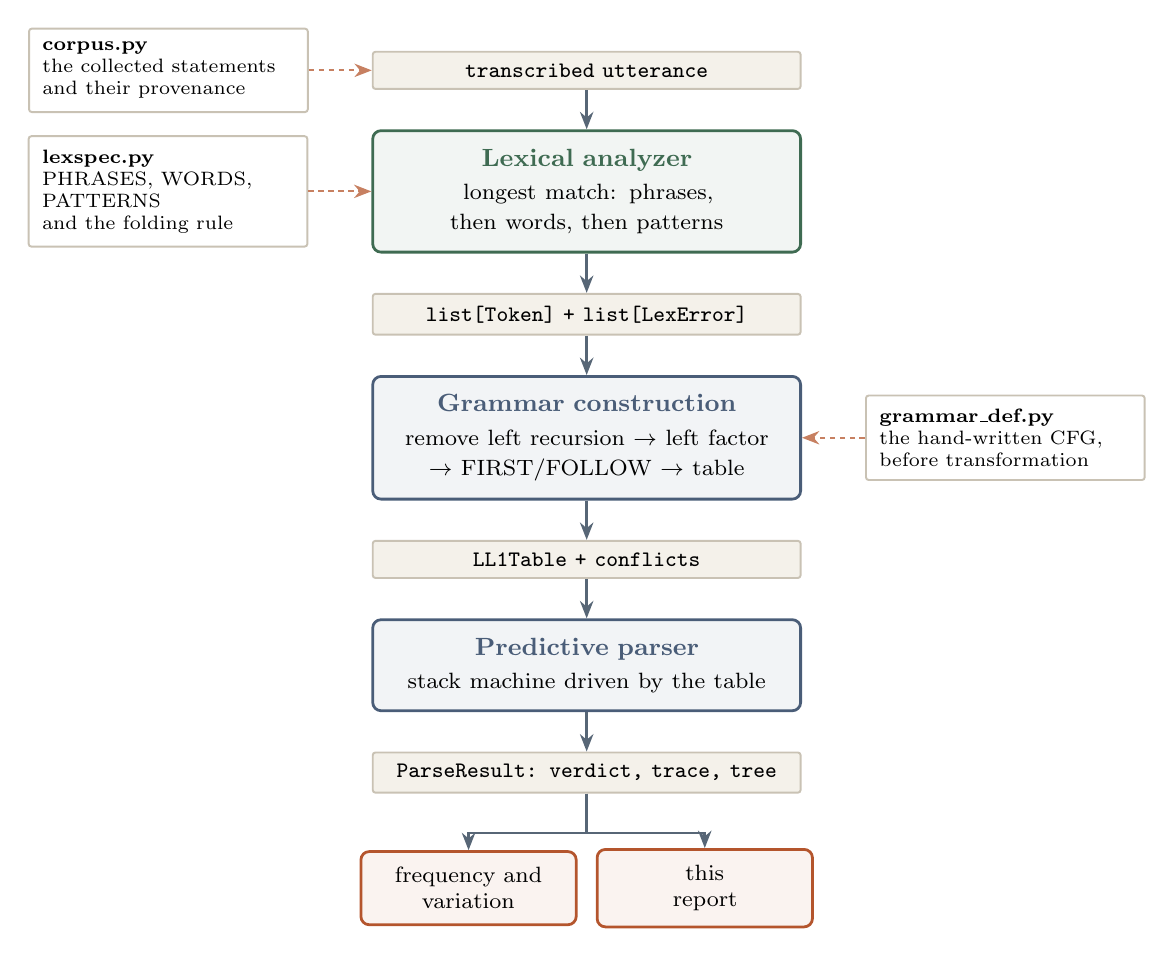
\begin{tikzpicture}[
  font=\small,
  node distance=5mm,
  >={Stealth[length=2.2mm,width=1.7mm]},
  data/.style={draw=rule, fill=parchment, line width=0.7pt,
               rounded corners=1pt, text width=52mm, align=center,
               font=\footnotesize\ttfamily, inner ysep=1.5mm},
  lex/.style={draw=moss, fill=moss!7, line width=1pt, rounded corners=3pt,
              text width=52mm, align=center, inner ysep=2.3mm},
  syn/.style={draw=slate, fill=slate!7, line width=1pt, rounded corners=3pt,
              text width=52mm, align=center, inner ysep=2.3mm},
  sink/.style={draw=clay, fill=clay!7, line width=1pt, rounded corners=3pt,
               text width=25mm, align=center, font=\footnotesize,
               inner ysep=2mm},
  spec/.style={draw=rule, fill=white, line width=0.7pt, rounded corners=1pt,
               text width=32mm, align=left, font=\scriptsize, inner sep=1.7mm},
  flow/.style={->, line width=1pt, draw=ink!75},
  feed/.style={->, line width=0.7pt, draw=clay!75, dash pattern=on 2pt off 1.6pt},
]

\node[data] (src) {transcribed utterance};

\node[lex, below=of src] (lexer)
  {\textbf{\color{moss}Lexical analyzer}\\[1pt]
   {\footnotesize longest match: phrases, then words, then patterns}};

\node[data, below=of lexer] (toks) {list[Token] + list[LexError]};

\node[syn, below=of toks] (gram)
  {\textbf{\color{slate}Grammar construction}\\[1pt]
   {\footnotesize remove left recursion \ensuremath{\rightarrow} left factor
    \ensuremath{\rightarrow} FIRST/FOLLOW \ensuremath{\rightarrow} table}};

\node[data, below=of gram] (tab) {LL1Table + conflicts};

\node[syn, below=of tab] (parser)
  {\textbf{\color{slate}Predictive parser}\\[1pt]
   {\footnotesize stack machine driven by the table}};

\node[data, below=of parser] (res) {ParseResult: verdict, trace, tree};

\node[sink] (stats) at ([xshift=-15mm,yshift=-12mm]res.south)
  {frequency and\\ variation};
\node[sink] (doc) at ([xshift=15mm,yshift=-12mm]res.south)
  {this\\ report};

\foreach \a/\b in {src/lexer, lexer/toks, toks/gram, gram/tab,
                   tab/parser, parser/res}
  \draw[flow] (\a) -- (\b);

\draw[flow] (res.south) -- ++(0,-5mm) -| (stats.north);
\draw[flow] (res.south) -- ++(0,-5mm) -| (doc.north);

\node[spec, left=8mm of lexer] (ls)
  {\textbf{lexspec.py}\\ PHRASES, WORDS, PATTERNS\\ and the folding rule};
\draw[feed] (ls) -- (lexer);

\node[spec, right=8mm of gram] (gs)
  {\textbf{grammar\_def.py}\\ the hand-written CFG,\\ before transformation};
\draw[feed] (gs) -- (gram);

\node[spec, left=8mm of src] (cs)
  {\textbf{corpus.py}\\ the collected statements\\ and their provenance};
\draw[feed] (cs) -- (src);

\end{tikzpicture}

\captionof{figure}{The analyzer pipeline. Solid arrows carry values; dashed
arrows are declarative inputs the stages consult.}
\end{center}

The two dashed inputs are the point of the design. The lexical specification and the grammar are data, not code paths: they are consulted by the stages rather than embedded in them. Changing either changes the analyzer's behaviour and, because every figure in this document is computed at generation time, changes this report with it.

\subsection{Modules}
\begingroup
\small
\rowcolors{1}{}{zebra}
\begin{longtable}{L{0.17} L{0.62}}
\caption{Modules and their responsibilities.}\\
\toprule
\rowcolor{headfill}\textbf{\color{ink}Module} & \textbf{\color{ink}Responsibility} \\
\midrule
\endfirsthead
\caption[]{Modules and their responsibilities. \textit{(continued)}}\\
\toprule
\rowcolor{headfill}\textbf{\color{ink}Module} & \textbf{\color{ink}Responsibility} \\
\midrule
\endhead
\midrule
\multicolumn{2}{r}{\footnotesize\textit{\color{slate}continued on the next page}}\\
\endfoot
\bottomrule
\endlastfoot
tokens.py & Token types, source languages, and the immutable Token record carrying both the original lexeme and its folded form. \\
lexspec.py & The lexical specification: multiword phrases, the closed vocabulary, the ordered regular expressions, and the folding rule. The single source of truth for tokenization. \\
lexer.py & Applies the specification, longest match first, and reports anything it cannot classify. \\
corpus.py & The collected statements with their metadata and provenance, plus the constructed negative tests. \\
grammar.py & Grammar representation and the algorithms: left-recursion removal, left factoring, FIRST, FOLLOW, table construction. \\
grammar\_def.py & The grammar itself, and the record of which conflicts have been reviewed. \\
parser.py & The predictive stack machine, the trace and the parse tree. \\
pipeline.py & Joins lexer and parser, producing one result per statement. \\
analysis.py & Frequency, spelling variation and code-mixing statistics. \\
report.py & Generates this document. \\
cli.py & The command-line interface. \\
\end{longtable}
\endgroup

One design decision deserves comment. The grammar transformations are implemented rather than done by hand and pasted in. This costs more code, but it means Sections 13 and 14 show what the program actually did, and that changing the grammar in one place updates the transformations, the FIRST and FOLLOW sets, the parse table and every trace in this report at once. A report that is written by hand alongside a program will eventually contradict it.

\section{Lexical analysis: the token inventory}
A token type is the category the parser sees: it is a terminal symbol of the grammar. Information that is linguistically interesting but syntactically irrelevant --- whether an item is slang, and which languages it draws on --- is carried alongside the token as annotation rather than folded into its type. Keeping the two apart allows a slang noun and a French noun to behave identically during parsing while still being counted separately in the frequency analysis.

\begingroup
\small
\rowcolors{1}{}{zebra}
\begin{longtable}{L{0.12} L{0.44} L{0.29}}
\caption{Terminal symbols of the grammar.}\\
\toprule
\rowcolor{headfill}\textbf{\color{ink}Token} & \textbf{\color{ink}Description} & \textbf{\color{ink}Examples} \\
\midrule
\endfirsthead
\caption[]{Terminal symbols of the grammar. \textit{(continued)}}\\
\toprule
\rowcolor{headfill}\textbf{\color{ink}Token} & \textbf{\color{ink}Description} & \textbf{\color{ink}Examples} \\
\midrule
\endhead
\midrule
\multicolumn{3}{r}{\footnotesize\textit{\color{slate}continued on the next page}}\\
\endfoot
\bottomrule
\endlastfoot
VOC & vocative or address term & Chef, Mami, Mbom \\
NOUN & noun, including place and operator names & quartier, reseau, Mokolo \\
PRON & pronoun & me, we, am \\
DET & determiner & this, ma, your \\
NUM & numeral or money amount & deux cents, 500 \\
ADJ & adjective & cher, long, zero-zero \\
ADV & adverbial & today, small small, trop \\
VERB & lexical verb & drop, hala, finish \\
AUX & aspect or modal marker & don, dey, make \\
NEG & negation & no, pas \\
PREP & preposition or directional marker & for, since, go \\
COP & copula & na, c'est \\
CONJ & coordinator & and, et \\
INTERJ & interjection or discourse cry & hmmm, ekiee, je wanda \\
PART & post-nominal particle & la, o \\
SEP & internal separator & , ; \\
TERM & sentence terminator & . ! ? \\
UNKNOWN & outside the specification, always reported & --- \\
\end{longtable}
\endgroup

\subsection{Declared vocabulary}
The specification declares 306 single-word entries and 24 multiword entries, distributed as follows.

\begingroup
\small
\rowcolors{1}{}{zebra}
\begin{longtable}{L{0.18} L{0.18}}
\caption{Size of the declared lexicon, by token type.}\\
\toprule
\rowcolor{headfill}\textbf{\color{ink}Token type} & \textbf{\color{ink}Declared entries} \\
\midrule
\endfirsthead
\caption[]{Size of the declared lexicon, by token type. \textit{(continued)}}\\
\toprule
\rowcolor{headfill}\textbf{\color{ink}Token type} & \textbf{\color{ink}Declared entries} \\
\midrule
\endhead
\midrule
\multicolumn{2}{r}{\footnotesize\textit{\color{slate}continued on the next page}}\\
\endfoot
\bottomrule
\endlastfoot
ADJ & 24 \\
ADV & 20 \\
AUX & 12 \\
CONJ & 9 \\
COP & 8 \\
DET & 27 \\
INTERJ & 22 \\
NEG & 4 \\
NOUN & 84 \\
NUM & 22 \\
PART & 2 \\
PREP & 18 \\
PRON & 22 \\
VERB & 48 \\
VOC & 8 \\
\end{longtable}
\endgroup

\section{Lexical specification: regular expressions}
The lexer applies three layers in a fixed order, and the order is part of the specification. Multiword lexemes are tried first, then the closed vocabulary, then the regular expressions. Within the first layer the longest candidate wins.

\begingroup
\footnotesize
\rowcolors{1}{}{zebra}
\begin{longtable}{L{0.14} L{0.50} L{0.19}}
\caption{Lexical rules, in application order.}\\
\toprule
\rowcolor{headfill}\textbf{\color{ink}Rule} & \textbf{\color{ink}Regular expression or method} & \textbf{\color{ink}Token type} \\
\midrule
\endfirsthead
\caption[]{Lexical rules, in application order. \textit{(continued)}}\\
\toprule
\rowcolor{headfill}\textbf{\color{ink}Rule} & \textbf{\color{ink}Regular expression or method} & \textbf{\color{ink}Token type} \\
\midrule
\endhead
\midrule
\multicolumn{3}{r}{\footnotesize\textit{\color{slate}continued on the next page}}\\
\endfoot
\bottomrule
\endlastfoot
R-PHRASE & \texttt{l\allowbreak{}o\allowbreak{}n\allowbreak{}g\allowbreak{}e\allowbreak{}s\allowbreak{}t\allowbreak{} \allowbreak{}m\allowbreak{}u\allowbreak{}l\allowbreak{}t\allowbreak{}i\allowbreak{}w\allowbreak{}o\allowbreak{}r\allowbreak{}d\allowbreak{} \allowbreak{}e\allowbreak{}n\allowbreak{}t\allowbreak{}r\allowbreak{}y\allowbreak{} \allowbreak{}f\allowbreak{}r\allowbreak{}o\allowbreak{}m\allowbreak{} \allowbreak{}P\allowbreak{}H\allowbreak{}R\allowbreak{}A\allowbreak{}S\allowbreak{}E\allowbreak{}S} & various \\
R-VOCAB & \texttt{e\allowbreak{}x\allowbreak{}a\allowbreak{}c\allowbreak{}t\allowbreak{} \allowbreak{}m\allowbreak{}a\allowbreak{}t\allowbreak{}c\allowbreak{}h\allowbreak{} \allowbreak{}a\allowbreak{}g\allowbreak{}a\allowbreak{}i\allowbreak{}n\allowbreak{}s\allowbreak{}t\allowbreak{} \allowbreak{}W\allowbreak{}O\allowbreak{}R\allowbreak{}D\allowbreak{}S\allowbreak{} \allowbreak{}a\allowbreak{}f\allowbreak{}t\allowbreak{}e\allowbreak{}r\allowbreak{} \allowbreak{}f\allowbreak{}o\allowbreak{}l\allowbreak{}d\allowbreak{}i\allowbreak{}n\allowbreak{}g} & various \\
R-MONEY & \texttt{\textbackslash\{\}\allowbreak{}d\allowbreak{}\{\allowbreak{}1\allowbreak{},\allowbreak{}3\allowbreak{}\}\allowbreak{}(\allowbreak{}?\allowbreak{}:\allowbreak{}[\allowbreak{} \allowbreak{}.\allowbreak{}]\allowbreak{}\textbackslash\{\}\allowbreak{}d\allowbreak{}\{\allowbreak{}3\allowbreak{}\}\allowbreak{})\allowbreak{}+\allowbreak{}|\allowbreak{}\textbackslash\{\}\allowbreak{}d\allowbreak{}+\allowbreak{}\textbackslash\{\}\allowbreak{}s\allowbreak{}*\allowbreak{}(\allowbreak{}?\allowbreak{}:\allowbreak{}f\allowbreak{}r\allowbreak{}s\allowbreak{}?\allowbreak{}|\allowbreak{}f\allowbreak{}c\allowbreak{}f\allowbreak{}a\allowbreak{}|\allowbreak{}f\allowbreak{}r\allowbreak{}a\allowbreak{}n\allowbreak{}c\allowbreak{}s\allowbreak{}?\allowbreak{})\allowbreak{}\textbackslash\{\}\allowbreak{}b} & NUM \\
R-NUM & \texttt{\textbackslash\{\}\allowbreak{}d\allowbreak{}+} & NUM \\
R-TERM & \texttt{[\allowbreak{}.\allowbreak{}!\allowbreak{}?\allowbreak{}]\allowbreak{}+} & TERM \\
R-SEP & \texttt{[\allowbreak{},\allowbreak{};\allowbreak{}:\allowbreak{}]} & SEP \\
R-INTERJ & \texttt{(\allowbreak{}?\allowbreak{}:\allowbreak{}h\allowbreak{}?\allowbreak{}m\allowbreak{}\{\allowbreak{}2\allowbreak{},\allowbreak{}\}\allowbreak{}|\allowbreak{}a\allowbreak{}\{\allowbreak{}2\allowbreak{},\allowbreak{}\}\allowbreak{}h\allowbreak{}+\allowbreak{}|\allowbreak{}e\allowbreak{}\{\allowbreak{}2\allowbreak{},\allowbreak{}\}\allowbreak{}h\allowbreak{}+\allowbreak{}|\allowbreak{}h\allowbreak{}+\allowbreak{}m\allowbreak{}+\allowbreak{}|\allowbreak{}w\allowbreak{}[\allowbreak{}e\allowbreak{}o\allowbreak{}]\allowbreak{}\{\allowbreak{}2\allowbreak{},\allowbreak{}\}\allowbreak{}h\allowbreak{}*\allowbreak{})} & INTERJ \\
R-SLANG-LONG & \texttt{[\allowbreak{}a\allowbreak{}-\allowbreak{}z\allowbreak{}]\allowbreak{}*\allowbreak{}(\allowbreak{}[\allowbreak{}a\allowbreak{}-\allowbreak{}z\allowbreak{}]\allowbreak{})\allowbreak{}\textbackslash\{\}\allowbreak{}1\allowbreak{}\{\allowbreak{}2\allowbreak{},\allowbreak{}\}\allowbreak{}[\allowbreak{}a\allowbreak{}-\allowbreak{}z\allowbreak{}]\allowbreak{}*} & INTERJ \\
R-WORD & \texttt{[\allowbreak{}A\allowbreak{}-\allowbreak{}Z\allowbreak{}a\allowbreak{}-\allowbreak{}z\allowbreak{}À\allowbreak{}-\allowbreak{}ÿ\allowbreak{}]\allowbreak{}+\allowbreak{}(\allowbreak{}?\allowbreak{}:\allowbreak{}[\allowbreak{}'\allowbreak{}\textbackslash\{\}\allowbreak{}u\allowbreak{}2\allowbreak{}0\allowbreak{}1\allowbreak{}9\allowbreak{}-\allowbreak{}]\allowbreak{}[\allowbreak{}A\allowbreak{}-\allowbreak{}Z\allowbreak{}a\allowbreak{}-\allowbreak{}z\allowbreak{}À\allowbreak{}-\allowbreak{}ÿ\allowbreak{}]\allowbreak{}+\allowbreak{})\allowbreak{}*} & UNKNOWN \\
\end{longtable}
\endgroup

\subsection{Why multiword lexemes are matched first}
Several expressions in this register are single lexical items that happen to be written as more than one word. ``Small small'' is not ``small'' twice: it is an adverbial meaning intermittently. ``Je wanda'' is not the French pronoun je followed by a verb: it is a fixed Camfranglais exclamation. ``Deux cents'' is one money amount. If the lexer matched word by word it would produce a token sequence that no reasonable grammar could interpret, so phrase matching runs before word matching and prefers the longest match. This is the same maximal-munch principle by which a conventional lexer prefers a keyword over its prefix.

\subsection{Productive patterns}
Two classes cannot be enumerated and are therefore handled by pattern. Hesitation and exasperation cries are productive --- a speaker may lengthen them arbitrarily --- so the rule R-INTERJ matches runs such as hmm, hmmm, aaah and eeeh. Emphatic slang lengthening is handled by R-SLANG-LONG, which matches any word containing a letter repeated three or more times, capturing garrr and its variants without listing each one.

\subsection{Unrecognised input}
Anything the three layers do not cover is emitted as an UNKNOWN token and recorded as a lexical error carrying its line and column. It is never silently discarded. The parser refuses any token stream containing UNKNOWN, which is why a lexical failure and a syntactic failure are reported as different kinds of rejection throughout this report.

\subsection{Relation to finite automata}
A conventional lexer compiles its regular expressions into a single deterministic finite automaton and runs the input through it once, remembering the last accepting state in order to implement maximal munch. The specification here is equivalent in expressive power --- every rule is regular, and the dictionary layers are finite sets, which are trivially regular --- but it is implemented as ordered dictionary lookup followed by regular-expression matching rather than as one combined automaton.

This is a deliberate trade. A combined automaton would be faster, but the specification would stop being readable: the point of this artefact is that a reader can see which rule classified which word, and the rule column of every token table in Section 8 depends on that being recoverable. At corpus scale the performance difference is irrelevant, and the priority is that the classification be auditable.

\subsection{A worked lexical trace}
Taking 'Chef, drop me for Carrefour Obili.', the lexer proceeds left to right. At each position it first tries the longest multiword entry that could start there, then a single-word entry, then the patterns in order. The first column below is the position in the input; the last names the rule that succeeded.

\begingroup
\footnotesize
\rowcolors{1}{}{zebra}
\begin{longtable}{L{0.07} L{0.17} L{0.11} L{0.11} L{0.30}}
\caption{Lexical decisions for one statement, in order.}\\
\toprule
\rowcolor{headfill}\textbf{\color{ink}Offset} & \textbf{\color{ink}Lexeme} & \textbf{\color{ink}Token} & \textbf{\color{ink}Rule} & \textbf{\color{ink}Decision} \\
\midrule
\endfirsthead
\caption[]{Lexical decisions for one statement, in order. \textit{(continued)}}\\
\toprule
\rowcolor{headfill}\textbf{\color{ink}Offset} & \textbf{\color{ink}Lexeme} & \textbf{\color{ink}Token} & \textbf{\color{ink}Rule} & \textbf{\color{ink}Decision} \\
\midrule
\endhead
\midrule
\multicolumn{5}{r}{\footnotesize\textit{\color{slate}continued on the next page}}\\
\endfoot
\bottomrule
\endlastfoot
0--4 & Chef & VOC & R-VOCAB & no dictionary entry; matched by pattern \\
4--5 & , & SEP & R-SEP & no dictionary entry; matched by pattern \\
6--10 & drop & VERB & R-VOCAB & no dictionary entry; matched by pattern \\
11--13 & me & PRON & R-VOCAB & no dictionary entry; matched by pattern \\
14--17 & for & PREP & R-VOCAB & no dictionary entry; matched by pattern \\
18--27 & Carrefour & NOUN & R-VOCAB & no dictionary entry; matched by pattern \\
28--33 & Obili & NOUN & R-VOCAB & no dictionary entry; matched by pattern \\
33--34 & . & TERM & R-TERM & no dictionary entry; matched by pattern \\
\end{longtable}
\endgroup

\section{Token tables, statement by statement}
The table below is the exact output of the lexical analyzer for every collected statement, in order. The rule column names the lexical rule that matched, so each classification can be traced back to the specification of Section 6. A bold line introduces each statement.

\begingroup
\scriptsize
\rowcolors{1}{}{zebra}
\begin{longtable}{L{0.03} L{0.13} L{0.07} L{0.12} L{0.04} L{0.08} L{0.28}}
\caption{Lexical analysis of every collected statement.}\\
\toprule
\rowcolor{headfill}\textbf{\color{ink}\#} & \textbf{\color{ink}Lexeme} & \textbf{\color{ink}Token} & \textbf{\color{ink}Language} & \textbf{\color{ink}Slang} & \textbf{\color{ink}Rule} & \textbf{\color{ink}Gloss} \\
\midrule
\endfirsthead
\caption[]{Lexical analysis of every collected statement. \textit{(continued)}}\\
\toprule
\rowcolor{headfill}\textbf{\color{ink}\#} & \textbf{\color{ink}Lexeme} & \textbf{\color{ink}Token} & \textbf{\color{ink}Language} & \textbf{\color{ink}Slang} & \textbf{\color{ink}Rule} & \textbf{\color{ink}Gloss} \\
\midrule
\endhead
\midrule
\multicolumn{7}{r}{\footnotesize\textit{\color{slate}continued on the next page}}\\
\endfoot
\bottomrule
\endlastfoot
\multicolumn{7}{@{}l@{}}{\rule{0pt}{2.6ex}\textbf{S01} Chef, drop me for Carrefour Obili. \textit{(ACCEPTED)}} \\
1 & Chef & VOC & French &  & R-VOCAB & boss, sir \\
2 & , & SEP & Symbol &  & R-SEP &  \\
3 & drop & VERB & English &  & R-VOCAB &  \\
4 & me & PRON & English &  & R-VOCAB &  \\
5 & for & PREP & English &  & R-VOCAB &  \\
6 & Carrefour & NOUN & French &  & R-VOCAB &  \\
7 & Obili & NOUN & ProperName &  & R-VOCAB & Yaounde neighbourhood or landmark \\
8 & . & TERM & Symbol &  & R-TERM &  \\
\multicolumn{7}{@{}l@{}}{\rule{0pt}{2.6ex}\textbf{S02} Patron, deux cents na for Mvan? \textit{(ACCEPTED)}} \\
1 & Patron & VOC & French &  & R-VOCAB & boss, sir \\
2 & , & SEP & Symbol &  & R-SEP &  \\
3 & deux cents & NUM & French &  & R-PHRASE & two hundred francs \\
4 & na & COP & Pidgin &  & R-VOCAB & equative copula: it is \\
5 & for & PREP & English &  & R-VOCAB &  \\
6 & Mvan & NOUN & ProperName &  & R-VOCAB & Yaounde neighbourhood or landmark \\
7 & ? & TERM & Symbol &  & R-TERM &  \\
\multicolumn{7}{@{}l@{}}{\rule{0pt}{2.6ex}\textbf{S03} Hmmm, chef, this road don cut, pay cinq cents. \textit{(ACCEPTED)}} \\
1 & Hmmm & INTERJ & Pidgin & yes & R-VOCAB & hesitation or exasperation cry \\
2 & , & SEP & Symbol &  & R-SEP &  \\
3 & chef & VOC & French &  & R-VOCAB & boss, sir \\
4 & , & SEP & Symbol &  & R-SEP &  \\
5 & this & DET & English &  & R-VOCAB &  \\
6 & road & NOUN & English &  & R-VOCAB &  \\
7 & don & AUX & Pidgin &  & R-VOCAB & perfective / progressive aspect marker \\
8 & cut & VERB & English &  & R-VOCAB &  \\
9 & , & SEP & Symbol &  & R-SEP &  \\
10 & pay & VERB & English &  & R-VOCAB &  \\
11 & cinq cents & NUM & French &  & R-PHRASE & five hundred francs \\
12 & . & TERM & Symbol &  & R-TERM &  \\
\multicolumn{7}{@{}l@{}}{\rule{0pt}{2.6ex}\textbf{S04} Ekiee, this MTN reseau dey small small today. \textit{(ACCEPTED)}} \\
1 & Ekiee & INTERJ & Ewondo & yes & R-VOCAB & Ewondo cry of shock or dismay \\
2 & , & SEP & Symbol &  & R-SEP &  \\
3 & this & DET & English &  & R-VOCAB &  \\
4 & MTN & NOUN & ProperName &  & R-VOCAB & utility or telecom operator \\
5 & reseau & NOUN & French &  & R-VOCAB &  \\
6 & dey & AUX & Pidgin &  & R-VOCAB & perfective / progressive aspect marker \\
7 & small small & ADV & Pidgin &  & R-PHRASE & little by little, intermittently \\
8 & today & ADV & English &  & R-VOCAB &  \\
9 & . & TERM & Symbol &  & R-TERM &  \\
\multicolumn{7}{@{}l@{}}{\rule{0pt}{2.6ex}\textbf{S05} Je wanda, my forfait don finish! \textit{(ACCEPTED)}} \\
1 & Je wanda & INTERJ & Pidgin/French & yes & R-PHRASE & I am amazed / unbelievable \\
2 & , & SEP & Symbol &  & R-SEP &  \\
3 & my & DET & English &  & R-VOCAB &  \\
4 & forfait & NOUN & French &  & R-VOCAB &  \\
5 & don & AUX & Pidgin &  & R-VOCAB & perfective / progressive aspect marker \\
6 & finish & VERB & English &  & R-VOCAB &  \\
7 & ! & TERM & Symbol &  & R-TERM &  \\
\multicolumn{7}{@{}l@{}}{\rule{0pt}{2.6ex}\textbf{S06} Garrr, ENEO don cut courant since ce matin. \textit{(ACCEPTED)}} \\
1 & Garrr & INTERJ & Camfranglais & yes & R-VOCAB & emphatic street exclamation \\
2 & , & SEP & Symbol &  & R-SEP &  \\
3 & ENEO & NOUN & ProperName &  & R-VOCAB & utility or telecom operator \\
4 & don & AUX & Pidgin &  & R-VOCAB & perfective / progressive aspect marker \\
5 & cut & VERB & English &  & R-VOCAB &  \\
6 & courant & NOUN & French &  & R-VOCAB &  \\
7 & since & PREP & English &  & R-VOCAB &  \\
8 & ce matin & NOUN & French &  & R-PHRASE & this morning \\
9 & . & TERM & Symbol &  & R-TERM &  \\
\multicolumn{7}{@{}l@{}}{\rule{0pt}{2.6ex}\textbf{S07} Courant no dey, we dey wait la nuit. \textit{(ACCEPTED)}} \\
1 & Courant & NOUN & French &  & R-VOCAB &  \\
2 & no & NEG & English &  & R-VOCAB &  \\
3 & dey & AUX & Pidgin &  & R-VOCAB & perfective / progressive aspect marker \\
4 & , & SEP & Symbol &  & R-SEP &  \\
5 & we & PRON & English &  & R-VOCAB &  \\
6 & dey & AUX & Pidgin &  & R-VOCAB & perfective / progressive aspect marker \\
7 & wait & VERB & English &  & R-VOCAB &  \\
8 & la nuit & NOUN & French &  & R-PHRASE & the night \\
9 & . & TERM & Symbol &  & R-TERM &  \\
\multicolumn{7}{@{}l@{}}{\rule{0pt}{2.6ex}\textbf{S08} Mami, reduce this tomate small, na trop cher. \textit{(ACCEPTED)}} \\
1 & Mami & VOC & Pidgin &  & R-VOCAB & market woman, mother \\
2 & , & SEP & Symbol &  & R-SEP &  \\
3 & reduce & VERB & English &  & R-VOCAB &  \\
4 & this & DET & English &  & R-VOCAB &  \\
5 & tomate & NOUN & French &  & R-VOCAB &  \\
6 & small & ADJ & Pidgin &  & R-VOCAB & small, a little \\
7 & , & SEP & Symbol &  & R-SEP &  \\
8 & na & COP & Pidgin &  & R-VOCAB & equative copula: it is \\
9 & trop & ADV & French &  & R-VOCAB &  \\
10 & cher & ADJ & French &  & R-VOCAB &  \\
11 & . & TERM & Symbol &  & R-TERM &  \\
\multicolumn{7}{@{}l@{}}{\rule{0pt}{2.6ex}\textbf{S09} Mbom, deux mille na last price o. \textit{(ACCEPTED)}} \\
1 & Mbom & VOC & Camfranglais & yes & R-VOCAB & Camfranglais address term: my friend, mate \\
2 & , & SEP & Symbol &  & R-SEP &  \\
3 & deux mille & NUM & French &  & R-PHRASE & two thousand francs \\
4 & na & COP & Pidgin &  & R-VOCAB & equative copula: it is \\
5 & last & ADJ & English &  & R-VOCAB &  \\
6 & price & NOUN & English &  & R-VOCAB &  \\
7 & o & PART & Pidgin &  & R-VOCAB & emphatic final particle \\
8 & . & TERM & Symbol &  & R-TERM &  \\
\multicolumn{7}{@{}l@{}}{\rule{0pt}{2.6ex}\textbf{S10} Weh, rain don beat we for Damas. \textit{(ACCEPTED)}} \\
1 & Weh & INTERJ & Pidgin & yes & R-VOCAB & cry of pity \\
2 & , & SEP & Symbol &  & R-SEP &  \\
3 & rain & NOUN & English &  & R-VOCAB &  \\
4 & don & AUX & Pidgin &  & R-VOCAB & perfective / progressive aspect marker \\
5 & beat & VERB & English &  & R-VOCAB &  \\
6 & we & PRON & English &  & R-VOCAB &  \\
7 & for & PREP & English &  & R-VOCAB &  \\
8 & Damas & NOUN & ProperName &  & R-VOCAB & Yaounde neighbourhood or landmark \\
9 & . & TERM & Symbol &  & R-TERM &  \\
\multicolumn{7}{@{}l@{}}{\rule{0pt}{2.6ex}\textbf{S11} This boue dey full the chemin, taxi no dey come. \textit{(ACCEPTED)}} \\
1 & This & DET & English &  & R-VOCAB &  \\
2 & boue & NOUN & French &  & R-VOCAB &  \\
3 & dey & AUX & Pidgin &  & R-VOCAB & perfective / progressive aspect marker \\
4 & full & ADJ & English &  & R-VOCAB &  \\
5 & the & DET & English &  & R-VOCAB &  \\
6 & chemin & NOUN & French &  & R-VOCAB &  \\
7 & , & SEP & Symbol &  & R-SEP &  \\
8 & taxi & NOUN & English &  & R-VOCAB &  \\
9 & no & NEG & English &  & R-VOCAB &  \\
10 & dey & AUX & Pidgin &  & R-VOCAB & perfective / progressive aspect marker \\
11 & come & VERB & English &  & R-VOCAB &  \\
12 & . & TERM & Symbol &  & R-TERM &  \\
\multicolumn{7}{@{}l@{}}{\rule{0pt}{2.6ex}\textbf{S12} Hmmm, queue for station dey long trop. \textit{(ACCEPTED)}} \\
1 & Hmmm & INTERJ & Pidgin & yes & R-VOCAB & hesitation or exasperation cry \\
2 & , & SEP & Symbol &  & R-SEP &  \\
3 & queue & NOUN & English &  & R-VOCAB &  \\
4 & for & PREP & English &  & R-VOCAB &  \\
5 & station & NOUN & French &  & R-VOCAB &  \\
6 & dey & AUX & Pidgin &  & R-VOCAB & perfective / progressive aspect marker \\
7 & long & ADJ & English &  & R-VOCAB &  \\
8 & trop & ADV & French &  & R-VOCAB &  \\
9 & . & TERM & Symbol &  & R-TERM &  \\
\multicolumn{7}{@{}l@{}}{\rule{0pt}{2.6ex}\textbf{S13} Bendskin man, carry me go Mokolo sharp sharp. \textit{(ACCEPTED)}} \\
1 & Bendskin man & VOC & Pidgin/French & yes & R-PHRASE & motorbike taxi rider \\
2 & , & SEP & Symbol &  & R-SEP &  \\
3 & carry & VERB & English &  & R-VOCAB &  \\
4 & me & PRON & English &  & R-VOCAB &  \\
5 & go & PREP & Pidgin &  & R-VOCAB & directional marker in serial verb constructions: carry me go Mokolo \\
6 & Mokolo & NOUN & ProperName &  & R-VOCAB & Yaounde neighbourhood or landmark \\
7 & sharp sharp & ADV & Pidgin & yes & R-PHRASE & immediately \\
8 & . & TERM & Symbol &  & R-TERM &  \\
\multicolumn{7}{@{}l@{}}{\rule{0pt}{2.6ex}\textbf{S14} Chef, bring your carte nationale! \textit{(ACCEPTED)}} \\
1 & Chef & VOC & French &  & R-VOCAB & boss, sir \\
2 & , & SEP & Symbol &  & R-SEP &  \\
3 & bring & VERB & English &  & R-VOCAB &  \\
4 & your & DET & English &  & R-VOCAB &  \\
5 & carte nationale & NOUN & French &  & R-PHRASE & national identity card \\
6 & ! & TERM & Symbol &  & R-TERM &  \\
\multicolumn{7}{@{}l@{}}{\rule{0pt}{2.6ex}\textbf{S15} Mola, the prof don drop resultats for lundi. \textit{(ACCEPTED)}} \\
1 & Mola & VOC & Camfranglais & yes & R-VOCAB & Camfranglais address term: my friend, mate \\
2 & , & SEP & Symbol &  & R-SEP &  \\
3 & the & DET & English &  & R-VOCAB &  \\
4 & prof & NOUN & French &  & R-VOCAB &  \\
5 & don & AUX & Pidgin &  & R-VOCAB & perfective / progressive aspect marker \\
6 & drop & VERB & English &  & R-VOCAB &  \\
7 & resultats & NOUN & French &  & R-VOCAB &  \\
8 & for & PREP & English &  & R-VOCAB &  \\
9 & lundi & NOUN & French &  & R-VOCAB &  \\
10 & . & TERM & Symbol &  & R-TERM &  \\
\end{longtable}
\endgroup

\subsection{The resulting token streams}
\begingroup
\scriptsize
\rowcolors{1}{}{zebra}
\begin{longtable}{L{0.05} L{0.76}}
\caption{The token stream handed to the parser for each statement.}\\
\toprule
\rowcolor{headfill}\textbf{\color{ink}ID} & \textbf{\color{ink}Token stream} \\
\midrule
\endfirsthead
\caption[]{The token stream handed to the parser for each statement. \textit{(continued)}}\\
\toprule
\rowcolor{headfill}\textbf{\color{ink}ID} & \textbf{\color{ink}Token stream} \\
\midrule
\endhead
\midrule
\multicolumn{2}{r}{\footnotesize\textit{\color{slate}continued on the next page}}\\
\endfoot
\bottomrule
\endlastfoot
S01 & \texttt{VOC SEP VERB PRON PREP NOUN NOUN TERM \$} \\
S02 & \texttt{VOC SEP NUM COP PREP NOUN TERM \$} \\
S03 & \texttt{INTERJ SEP VOC SEP DET NOUN AUX VERB SEP VERB NUM TERM \$} \\
S04 & \texttt{INTERJ SEP DET NOUN NOUN AUX ADV ADV TERM \$} \\
S05 & \texttt{INTERJ SEP DET NOUN AUX VERB TERM \$} \\
S06 & \texttt{INTERJ SEP NOUN AUX VERB NOUN PREP NOUN TERM \$} \\
S07 & \texttt{NOUN NEG AUX SEP PRON AUX VERB NOUN TERM \$} \\
S08 & \texttt{VOC SEP VERB DET NOUN ADJ SEP COP ADV ADJ TERM \$} \\
S09 & \texttt{VOC SEP NUM COP ADJ NOUN PART TERM \$} \\
S10 & \texttt{INTERJ SEP NOUN AUX VERB PRON PREP NOUN TERM \$} \\
S11 & \texttt{DET NOUN AUX ADJ DET NOUN SEP NOUN NEG AUX VERB TERM \$} \\
S12 & \texttt{INTERJ SEP NOUN PREP NOUN AUX ADJ ADV TERM \$} \\
S13 & \texttt{VOC SEP VERB PRON PREP NOUN ADV TERM \$} \\
S14 & \texttt{VOC SEP VERB DET NOUN TERM \$} \\
S15 & \texttt{VOC SEP DET NOUN AUX VERB NOUN PREP NOUN TERM \$} \\
\end{longtable}
\endgroup

\section{The complete lexical inventory of the corpus}
Collapsing the 134 tokens of Section 8 by token type and folded form leaves 76 distinct lexical items. This is the vocabulary the corpus actually exercises, as opposed to the vocabulary the specification declares, and the difference between the two is a measure of how much of the specification is currently evidenced by data.

\begingroup
\footnotesize
\rowcolors{1}{}{zebra}
\begin{longtable}{L{0.10} L{0.06} L{0.64}}
\caption{Every distinct lexical item attested in the corpus, grouped by token type.}\\
\toprule
\rowcolor{headfill}\textbf{\color{ink}Token} & \textbf{\color{ink}Count} & \textbf{\color{ink}Attested lexical items} \\
\midrule
\endfirsthead
\caption[]{Every distinct lexical item attested in the corpus, grouped by token type. \textit{(continued)}}\\
\toprule
\rowcolor{headfill}\textbf{\color{ink}Token} & \textbf{\color{ink}Count} & \textbf{\color{ink}Attested lexical items} \\
\midrule
\endhead
\midrule
\multicolumn{3}{r}{\footnotesize\textit{\color{slate}continued on the next page}}\\
\endfoot
\bottomrule
\endlastfoot
ADJ & 5 & cher, full, last, long, small \\
ADV & 4 & sharp sharp, small small, today, trop \\
AUX & 2 & dey, don \\
COP & 1 & na \\
DET & 4 & my, the, this, your \\
INTERJ & 5 & ekiee, garrr, hmmm, je wanda, weh \\
NEG & 1 & no \\
NOUN & 25 & boue, carrefour, carte nationale, ce matin, chemin, courant, damas, eneo, forfait, la nuit, lundi, mokolo, mtn, mvan, obili, price, prof, queue, rain, reseau, resultats, road, station, taxi, tomate \\
NUM & 3 & cinq cents, deux cents, deux mille \\
PART & 1 & o \\
PREP & 3 & for, go, since \\
PRON & 2 & me, we \\
SEP & 1 & , \\
TERM & 3 & !, ., ? \\
VERB & 10 & beat, bring, carry, come, cut, drop, finish, pay, reduce, wait \\
VOC & 6 & bendskin man, chef, mami, mbom, mola, patron \\
\end{longtable}
\endgroup

Glosses and source languages for each of these appear in Section 8, where every occurrence is listed with its statement.

The specification declares 330 entries and the corpus exercises 76 of them, or 23.0\%. The remainder were added during development because they are common in the register, but they are not attested in this corpus. They are honest coverage rather than evidence, and a larger corpus would be needed to justify them.

\section{Token frequency and variation}
The corpus yields 134 tokens over 76 distinct lexical items, a type/token ratio of 0.57.

\subsection{Frequency by token type}
\begingroup
\small
\rowcolors{1}{}{zebra}
\begin{longtable}{L{0.16} L{0.12} L{0.12}}
\caption{Distribution of terminal symbols across the corpus.}\\
\toprule
\rowcolor{headfill}\textbf{\color{ink}Token type} & \textbf{\color{ink}Count} & \textbf{\color{ink}Share} \\
\midrule
\endfirsthead
\caption[]{Distribution of terminal symbols across the corpus. \textit{(continued)}}\\
\toprule
\rowcolor{headfill}\textbf{\color{ink}Token type} & \textbf{\color{ink}Count} & \textbf{\color{ink}Share} \\
\midrule
\endhead
\midrule
\multicolumn{3}{r}{\footnotesize\textit{\color{slate}continued on the next page}}\\
\endfoot
\bottomrule
\endlastfoot
NOUN & 26 & 19.4\% \\
SEP & 18 & 13.4\% \\
TERM & 15 & 11.2\% \\
VERB & 12 & 9.0\% \\
AUX & 11 & 8.2\% \\
VOC & 8 & 6.0\% \\
DET & 8 & 6.0\% \\
PREP & 7 & 5.2\% \\
INTERJ & 6 & 4.5\% \\
ADV & 5 & 3.7\% \\
ADJ & 5 & 3.7\% \\
PRON & 4 & 3.0\% \\
NUM & 3 & 2.2\% \\
COP & 3 & 2.2\% \\
NEG & 2 & 1.5\% \\
PART & 1 & 0.7\% \\
\end{longtable}
\endgroup

\subsection{Most frequent lexical items}
\begingroup
\small
\rowcolors{1}{}{zebra}
\begin{longtable}{L{0.17} L{0.07} L{0.11} L{0.40}}
\caption{The most frequent lexical items.}\\
\toprule
\rowcolor{headfill}\textbf{\color{ink}Lexeme} & \textbf{\color{ink}Count} & \textbf{\color{ink}Token type} & \textbf{\color{ink}Spellings attested} \\
\midrule
\endfirsthead
\caption[]{The most frequent lexical items. \textit{(continued)}}\\
\toprule
\rowcolor{headfill}\textbf{\color{ink}Lexeme} & \textbf{\color{ink}Count} & \textbf{\color{ink}Token type} & \textbf{\color{ink}Spellings attested} \\
\midrule
\endhead
\midrule
\multicolumn{4}{r}{\footnotesize\textit{\color{slate}continued on the next page}}\\
\endfoot
\bottomrule
\endlastfoot
, & 18 & SEP & , (18) \\
. & 12 & TERM & . (12) \\
dey & 6 & AUX & dey (6) \\
for & 5 & PREP & for (5) \\
don & 5 & AUX & don (5) \\
this & 4 & DET & this (3), This (1) \\
chef & 3 & VOC & Chef (2), chef (1) \\
na & 3 & COP & na (3) \\
drop & 2 & VERB & drop (2) \\
me & 2 & PRON & me (2) \\
hmmm & 2 & INTERJ & Hmmm (2) \\
cut & 2 & VERB & cut (2) \\
! & 2 & TERM & ! (2) \\
courant & 2 & NOUN & courant (1), Courant (1) \\
no & 2 & NEG & no (2) \\
\end{longtable}
\endgroup

\subsection{Variation}
The following items are attested with more than one written form. They are counted as one lexical item, but every spelling is retained.

\begingroup
\small
\rowcolors{1}{}{zebra}
\begin{longtable}{L{0.17} L{0.07} L{0.07} L{0.44}}
\caption{Lexical items with more than one attested spelling.}\\
\toprule
\rowcolor{headfill}\textbf{\color{ink}Lexeme} & \textbf{\color{ink}Forms} & \textbf{\color{ink}Total} & \textbf{\color{ink}Attested spellings} \\
\midrule
\endfirsthead
\caption[]{Lexical items with more than one attested spelling. \textit{(continued)}}\\
\toprule
\rowcolor{headfill}\textbf{\color{ink}Lexeme} & \textbf{\color{ink}Forms} & \textbf{\color{ink}Total} & \textbf{\color{ink}Attested spellings} \\
\midrule
\endhead
\midrule
\multicolumn{4}{r}{\footnotesize\textit{\color{slate}continued on the next page}}\\
\endfoot
\bottomrule
\endlastfoot
this & 2 & 4 & this (3), This (1) \\
chef & 2 & 3 & Chef (2), chef (1) \\
courant & 2 & 2 & courant (1), Courant (1) \\
\end{longtable}
\endgroup

\subsection{Multiword lexemes recognised as single tokens}
\begingroup
\small
\rowcolors{1}{}{zebra}
\begin{longtable}{L{0.24} L{0.16}}
\caption{Multiword lexemes, each treated as one token.}\\
\toprule
\rowcolor{headfill}\textbf{\color{ink}Lexeme} & \textbf{\color{ink}Occurrences} \\
\midrule
\endfirsthead
\caption[]{Multiword lexemes, each treated as one token. \textit{(continued)}}\\
\toprule
\rowcolor{headfill}\textbf{\color{ink}Lexeme} & \textbf{\color{ink}Occurrences} \\
\midrule
\endhead
\midrule
\multicolumn{2}{r}{\footnotesize\textit{\color{slate}continued on the next page}}\\
\endfoot
\bottomrule
\endlastfoot
deux cents & 1 \\
cinq cents & 1 \\
small small & 1 \\
je wanda & 1 \\
ce matin & 1 \\
la nuit & 1 \\
deux mille & 1 \\
bendskin man & 1 \\
sharp sharp & 1 \\
carte nationale & 1 \\
\end{longtable}
\endgroup

\subsection{Slang and Camfranglais items}
\begingroup
\small
\rowcolors{1}{}{zebra}
\begin{longtable}{L{0.24} L{0.16}}
\caption{Items flagged as slang or Camfranglais.}\\
\toprule
\rowcolor{headfill}\textbf{\color{ink}Lexeme} & \textbf{\color{ink}Occurrences} \\
\midrule
\endfirsthead
\caption[]{Items flagged as slang or Camfranglais. \textit{(continued)}}\\
\toprule
\rowcolor{headfill}\textbf{\color{ink}Lexeme} & \textbf{\color{ink}Occurrences} \\
\midrule
\endhead
\midrule
\multicolumn{2}{r}{\footnotesize\textit{\color{slate}continued on the next page}}\\
\endfoot
\bottomrule
\endlastfoot
hmmm & 2 \\
ekiee & 1 \\
je wanda & 1 \\
garrr & 1 \\
mbom & 1 \\
weh & 1 \\
bendskin man & 1 \\
sharp sharp & 1 \\
mola & 1 \\
\end{longtable}
\endgroup

\section{Code-mixing analysis}
\subsection{Tokens by source language}
\begingroup
\small
\rowcolors{1}{}{zebra}
\begin{longtable}{L{0.20} L{0.18} L{0.12}}
\caption{Source languages drawn on across the corpus.}\\
\toprule
\rowcolor{headfill}\textbf{\color{ink}Language} & \textbf{\color{ink}Token attributions} & \textbf{\color{ink}Share} \\
\midrule
\endfirsthead
\caption[]{Source languages drawn on across the corpus. \textit{(continued)}}\\
\toprule
\rowcolor{headfill}\textbf{\color{ink}Language} & \textbf{\color{ink}Token attributions} & \textbf{\color{ink}Share} \\
\midrule
\endhead
\midrule
\multicolumn{3}{r}{\footnotesize\textit{\color{slate}continued on the next page}}\\
\endfoot
\bottomrule
\endlastfoot
English & 41 & 30.1\% \\
Symbol & 33 & 24.3\% \\
French & 27 & 19.9\% \\
Pidgin & 25 & 18.4\% \\
ProperName & 6 & 4.4\% \\
Camfranglais & 3 & 2.2\% \\
Ewondo & 1 & 0.7\% \\
\end{longtable}
\endgroup

A token may be attributed to more than one language, which is why the attribution count exceeds the token count. Those are the items that are themselves code-mixed rather than merely adjacent to another language.

\subsection{Statements drawing on more than one language}
\begingroup
\small
\rowcolors{1}{}{zebra}
\begin{longtable}{L{0.14} L{0.60}}
\caption{Code-mixing at the level of the statement.}\\
\toprule
\rowcolor{headfill}\textbf{\color{ink}Statement} & \textbf{\color{ink}Languages} \\
\midrule
\endfirsthead
\caption[]{Code-mixing at the level of the statement. \textit{(continued)}}\\
\toprule
\rowcolor{headfill}\textbf{\color{ink}Statement} & \textbf{\color{ink}Languages} \\
\midrule
\endhead
\midrule
\multicolumn{2}{r}{\footnotesize\textit{\color{slate}continued on the next page}}\\
\endfoot
\bottomrule
\endlastfoot
S01 & English, French, ProperName \\
S02 & English, French, Pidgin, ProperName \\
S03 & English, French, Pidgin \\
S04 & English, Ewondo, French, Pidgin, ProperName \\
S05 & English, French, Pidgin \\
S06 & Camfranglais, English, French, Pidgin, ProperName \\
S07 & English, French, Pidgin \\
S08 & English, French, Pidgin \\
S09 & Camfranglais, English, French, Pidgin \\
S10 & English, Pidgin, ProperName \\
S11 & English, French, Pidgin \\
S12 & English, French, Pidgin \\
S13 & English, French, Pidgin, ProperName \\
S14 & English, French \\
S15 & Camfranglais, English, French, Pidgin \\
\end{longtable}
\endgroup

15 of 15 statements draw on more than one language.

\section{Syntactic analysis: the grammar}
The grammar describes the shape of the utterances in the corpus. Read informally, a statement is an optional run of openers (interjections and address terms), then one or more clauses separated by commas, then a terminator:


\begin{center}
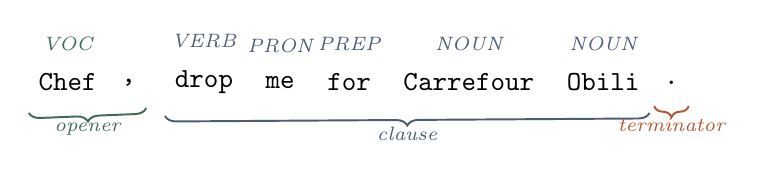
\begin{tikzpicture}[
  font=\small,
  lexeme/.style={font=\ttfamily, inner sep=1.2mm},
  brace/.style={decorate, decoration={brace, amplitude=4pt, raise=1.5pt},
                line width=0.7pt},
  tag/.style={font=\scriptsize\itshape, inner sep=0.8mm},
]

\node[lexeme] (w1) {Chef};
\node[lexeme, right=0.6mm of w1] (w2) {,};
\node[lexeme, right=2.4mm of w2] (w3) {drop};
\node[lexeme, right=1.6mm of w3] (w4) {me};
\node[lexeme, right=1.6mm of w4] (w5) {for};
\node[lexeme, right=1.6mm of w5] (w6) {Carrefour};
\node[lexeme, right=1.6mm of w6] (w7) {Obili};
\node[lexeme, right=0.6mm of w7] (w8) {.};

\draw[brace, draw=moss]
  ([yshift=-1mm]w2.south east) -- ([yshift=-1mm]w1.south west)
  node[tag, midway, below=3.5pt, color=moss] {opener};
\draw[brace, draw=slate]
  ([yshift=-1mm]w7.south east) -- ([yshift=-1mm]w3.south west)
  node[tag, midway, below=3.5pt, color=slate] {clause};
\draw[brace, draw=clay]
  ([yshift=-1mm]w8.south east) -- ([yshift=-1mm]w8.south west)
  node[tag, midway, below=3.5pt, color=clay] {terminator};

\node[tag, above=2.5pt of w1, color=moss] {VOC};
\node[tag, above=2.5pt of w3, color=slate] {VERB};
\node[tag, above=2.5pt of w4, color=slate] {PRON};
\node[tag, above=2.5pt of w5, color=slate] {PREP};
\node[tag, above=2.5pt of w6, color=slate] {NOUN};
\node[tag, above=2.5pt of w7, color=slate] {NOUN};

\end{tikzpicture}

\captionof{figure}{How the grammar decomposes a statement, with the token
type assigned to each lexeme.}
\end{center}

A clause is an optional subject followed by either a verbal predicate or a copular predicate. The verbal predicate may be headed by negation or by an aspect marker --- don for the perfective, dey for the progressive --- which is the Pidgin pattern rather than the English one, and the grammar encodes it directly.

The grammar as first written:

\begin{Verbatim}[commandchars=\\\{\},fontsize=\small,formatcom=\vbfmt,frame=leftline,framerule=1.2pt,rulecolor=\color{clay!55},framesep=6pt,xleftmargin=10pt,xrightmargin=4pt]
Statement  -> Preamble ClauseList TERM
Preamble   -> Opener Preamble | \eps{}
Opener     -> INTERJ SepOpt | VOC SepOpt
SepOpt     -> SEP | \eps{}
ClauseList -> ClauseList SEP Clause | Clause
Clause     -> Subj VP | Subj COP Items
Subj       -> NP SubjPP | \eps{}
SubjPP     -> PP | \eps{}
VP         -> NEG AuxSeq Core | AUX AuxSeq Core | VERB Items
AuxSeq     -> AUX AuxSeq | \eps{}
Core       -> VERB Items | Items
Items      -> Item Items | \eps{}
Item       -> ADJ | ADV | PART | NP | PP
NP         -> PRON | DET NGopt | NUM NGopt | NOUN NGopt
NGopt      -> NOUN NGopt | \eps{}
PP         -> PREP NP
\end{Verbatim}
Two properties of this grammar are deliberate, because the assignment requires the corresponding transformations. ClauseList is left recursive, which a predictive parser cannot handle. The two Clause productions share the prefix Subj, which prevents a one-token lookahead from choosing between them. The next two sections remove both.

\subsection{What each nonterminal stands for}
\begingroup
\small
\rowcolors{1}{}{zebra}
\begin{longtable}{L{0.15} L{0.66}}
\caption{The nonterminals of the final grammar.}\\
\toprule
\rowcolor{headfill}\textbf{\color{ink}Nonterminal} & \textbf{\color{ink}Meaning} \\
\midrule
\endfirsthead
\caption[]{The nonterminals of the final grammar. \textit{(continued)}}\\
\toprule
\rowcolor{headfill}\textbf{\color{ink}Nonterminal} & \textbf{\color{ink}Meaning} \\
\midrule
\endhead
\midrule
\multicolumn{2}{r}{\footnotesize\textit{\color{slate}continued on the next page}}\\
\endfoot
\bottomrule
\endlastfoot
Statement & A complete utterance: openers, clauses, terminator. \\
Preamble & The run of interjections and address terms that may precede the first clause. \\
Opener & One interjection or one vocative. \\
SepOpt & An optional comma after an opener. \\
ClauseList & One or more clauses separated by commas. \\
ClauseList' & Generated when left recursion was removed from ClauseList; carries the remaining comma-separated clauses. \\
Clause & A subject followed by a predicate. \\
Subj & An optional noun phrase, optionally modified by a prepositional phrase. Optional because subjects are freely dropped in this register. \\
SubjPP & The optional prepositional modifier of the subject; separated out to keep the parse table conflict-free. \\
VP & A verbal predicate, possibly headed by negation or aspect. \\
AuxSeq & A run of aspect and modal markers preceding the verb. \\
Core & The verb together with what follows it. \\
Items & A sequence of post-verbal or post-copular constituents. \\
Item & One such constituent: a noun phrase, a prepositional phrase, an adverbial or a numeral. \\
NP & A noun phrase: optional determiner, noun group, optional particle. \\
NGopt & The optional continuation of a noun compound; the source of the documented conflict in Section 18. \\
PP & A preposition followed by a noun phrase. \\
Clause\_f & Generated by left factoring; decides between the verbal and the copular predicate once the shared subject has been parsed. \\
\end{longtable}
\endgroup

\subsection{Design decisions behind the grammar}
The subject is optional. Statements such as ``Na wuna own.'' and ``Chef, drop me for Carrefour Obili.'' have no overt subject, and treating that as an error would reject a large share of the corpus. Subj therefore derives the empty string.

Aspect is a separate category. AUX covers don and dey, which mark completion and ongoing action. They are free morphemes preceding the verb, so they are modelled as a sequence AuxSeq rather than as inflection on the verb.

Negation may head the predicate. Both ``no dey'' and ``pas cher'' place the negator before what it negates, so VP admits a leading NEG.

Noun compounding is unbounded. Sequences such as ``carrefour Obili'' and ``bendskin man'' are nouns modifying nouns with no limit and no determiner between them, which is why NGopt is recursive --- and why it is the one place the grammar is ambiguous.

Clause structure is flat on purpose. Items makes no distinction between an argument and an adjunct. The distinction is real, but recovering it requires knowing what the verb means, which is semantic analysis and out of scope.

\section{Removing left recursion}
A production of the form A -> A alpha, alternating with A -> beta, causes a predictive parser to expand A into A forever without consuming input. It is removed by rewriting the pair as A -> beta A-prime together with A-prime -> alpha A-prime, alternating with the empty production. The rewritten grammar generates the same language while consuming beta before recursing.

ClauseList: immediate left recursion on ClauseList, introduced ClauseList'.

\begin{Verbatim}[commandchars=\\\{\},fontsize=\small,formatcom=\vbfmt,frame=leftline,framerule=1.2pt,rulecolor=\color{clay!55},framesep=6pt,xleftmargin=10pt,xrightmargin=4pt]
from:  ClauseList -> ClauseList SEP Clause
from:  ClauseList -> Clause
to:    ClauseList -> Clause ClauseList'
to:    ClauseList' -> SEP Clause ClauseList'
to:    ClauseList' -> \eps{}
\end{Verbatim}
The grammar after this step:

\begin{Verbatim}[commandchars=\\\{\},fontsize=\small,formatcom=\vbfmt,frame=leftline,framerule=1.2pt,rulecolor=\color{clay!55},framesep=6pt,xleftmargin=10pt,xrightmargin=4pt]
Statement   -> Preamble ClauseList TERM
Preamble    -> Opener Preamble | \eps{}
Opener      -> INTERJ SepOpt | VOC SepOpt
SepOpt      -> SEP | \eps{}
ClauseList  -> Clause ClauseList'
ClauseList' -> SEP Clause ClauseList' | \eps{}
Clause      -> Subj VP | Subj COP Items
Subj        -> NP SubjPP | \eps{}
SubjPP      -> PP | \eps{}
VP          -> NEG AuxSeq Core | AUX AuxSeq Core | VERB Items
AuxSeq      -> AUX AuxSeq | \eps{}
Core        -> VERB Items | Items
Items       -> Item Items | \eps{}
Item        -> ADJ | ADV | PART | NP | PP
NP          -> PRON | DET NGopt | NUM NGopt | NOUN NGopt
NGopt       -> NOUN NGopt | \eps{}
PP          -> PREP NP
\end{Verbatim}
\section{Left factoring}
When two productions of the same nonterminal begin with the same symbols, one token of lookahead cannot tell them apart. The common prefix is factored out into a single production and the differing tails move into a new nonterminal, which defers the decision until the parser has read enough to make it.

Clause: common prefix 'Subj', introduced Clause\_f.

\begin{Verbatim}[commandchars=\\\{\},fontsize=\small,formatcom=\vbfmt,frame=leftline,framerule=1.2pt,rulecolor=\color{clay!55},framesep=6pt,xleftmargin=10pt,xrightmargin=4pt]
from:  Clause -> Subj VP
from:  Clause -> Subj COP Items
to:    Clause -> Subj Clause_f
to:    Clause_f -> VP
to:    Clause_f -> COP Items
\end{Verbatim}
Concretely: on reading ``Courant ...'' the parser cannot yet know whether the clause continues ``... no dey'', which is verbal, or ``... na trop cher'', which is copular. After factoring it parses the shared subject first and decides at Clause\_f, by which point the next token settles the question.

The final grammar:

\begin{Verbatim}[commandchars=\\\{\},fontsize=\small,formatcom=\vbfmt,frame=leftline,framerule=1.2pt,rulecolor=\color{clay!55},framesep=6pt,xleftmargin=10pt,xrightmargin=4pt]
Statement   -> Preamble ClauseList TERM
Preamble    -> Opener Preamble | \eps{}
Opener      -> INTERJ SepOpt | VOC SepOpt
SepOpt      -> SEP | \eps{}
ClauseList  -> Clause ClauseList'
ClauseList' -> SEP Clause ClauseList' | \eps{}
Clause      -> Subj Clause_f
Subj        -> NP SubjPP | \eps{}
SubjPP      -> PP | \eps{}
VP          -> NEG AuxSeq Core | AUX AuxSeq Core | VERB Items
AuxSeq      -> AUX AuxSeq | \eps{}
Core        -> VERB Items | Items
Items       -> Item Items | \eps{}
Item        -> ADJ | ADV | PART | NP | PP
NP          -> PRON | DET NGopt | NUM NGopt | NOUN NGopt
NGopt       -> NOUN NGopt | \eps{}
PP          -> PREP NP
Clause_f    -> VP | COP Items
\end{Verbatim}
\subsection{Numbered productions}
\begin{Verbatim}[commandchars=\\\{\},fontsize=\small,formatcom=\vbfmt,frame=leftline,framerule=1.2pt,rulecolor=\color{clay!55},framesep=6pt,xleftmargin=10pt,xrightmargin=4pt]
 1. Statement -> Preamble ClauseList TERM
 2. Preamble -> Opener Preamble
 3. Preamble -> \eps{}
 4. Opener -> INTERJ SepOpt
 5. Opener -> VOC SepOpt
 6. SepOpt -> SEP
 7. SepOpt -> \eps{}
 8. ClauseList -> Clause ClauseList'
 9. ClauseList' -> SEP Clause ClauseList'
10. ClauseList' -> \eps{}
11. Clause -> Subj Clause_f
12. Subj -> NP SubjPP
13. Subj -> \eps{}
14. SubjPP -> PP
15. SubjPP -> \eps{}
16. VP -> NEG AuxSeq Core
17. VP -> AUX AuxSeq Core
18. VP -> VERB Items
19. AuxSeq -> AUX AuxSeq
20. AuxSeq -> \eps{}
21. Core -> VERB Items
22. Core -> Items
23. Items -> Item Items
24. Items -> \eps{}
25. Item -> ADJ
26. Item -> ADV
27. Item -> PART
28. Item -> NP
29. Item -> PP
30. NP -> PRON
31. NP -> DET NGopt
32. NP -> NUM NGopt
33. NP -> NOUN NGopt
34. NGopt -> NOUN NGopt
35. NGopt -> \eps{}
36. PP -> PREP NP
37. Clause_f -> VP
38. Clause_f -> COP Items
\end{Verbatim}
\section{FIRST and FOLLOW sets}
FIRST of a symbol X is the set of terminals that can begin a string derived from X, plus the empty production if X can derive it. FOLLOW of a nonterminal A is the set of terminals that can appear immediately after A in some derivation, with the dollar sign marking end of input. Both are computed by fixed-point iteration; the sets below are that computed result, not a transcription.

\begingroup
\footnotesize
\rowcolors{1}{}{zebra}
\begin{longtable}{L{0.13} L{0.36} L{0.36}}
\caption{FIRST and FOLLOW sets of the final grammar.}\\
\toprule
\rowcolor{headfill}\textbf{\color{ink}Nonterminal} & \textbf{\color{ink}FIRST} & \textbf{\color{ink}FOLLOW} \\
\midrule
\endfirsthead
\caption[]{FIRST and FOLLOW sets of the final grammar. \textit{(continued)}}\\
\toprule
\rowcolor{headfill}\textbf{\color{ink}Nonterminal} & \textbf{\color{ink}FIRST} & \textbf{\color{ink}FOLLOW} \\
\midrule
\endhead
\midrule
\multicolumn{3}{r}{\footnotesize\textit{\color{slate}continued on the next page}}\\
\endfoot
\bottomrule
\endlastfoot
Statement & \{ AUX, COP, DET, INTERJ, NEG, NOUN, NUM, PRON, VERB, VOC \} & \{ \$ \} \\
Preamble & \{ INTERJ, VOC, \eps{} \} & \{ AUX, COP, DET, NEG, NOUN, NUM, PRON, VERB \} \\
Opener & \{ INTERJ, VOC \} & \{ AUX, COP, DET, INTERJ, NEG, NOUN, NUM, PRON, VERB, VOC \} \\
SepOpt & \{ SEP, \eps{} \} & \{ AUX, COP, DET, INTERJ, NEG, NOUN, NUM, PRON, VERB, VOC \} \\
ClauseList & \{ AUX, COP, DET, NEG, NOUN, NUM, PRON, VERB \} & \{ TERM \} \\
ClauseList' & \{ SEP, \eps{} \} & \{ TERM \} \\
Clause & \{ AUX, COP, DET, NEG, NOUN, NUM, PRON, VERB \} & \{ SEP, TERM \} \\
Subj & \{ DET, NOUN, NUM, PRON, \eps{} \} & \{ AUX, COP, NEG, VERB \} \\
SubjPP & \{ PREP, \eps{} \} & \{ AUX, COP, NEG, VERB \} \\
VP & \{ AUX, NEG, VERB \} & \{ SEP, TERM \} \\
AuxSeq & \{ AUX, \eps{} \} & \{ ADJ, ADV, DET, NOUN, NUM, PART, PREP, PRON, SEP, TERM, VERB \} \\
Core & \{ ADJ, ADV, DET, NOUN, NUM, PART, PREP, PRON, VERB, \eps{} \} & \{ SEP, TERM \} \\
Items & \{ ADJ, ADV, DET, NOUN, NUM, PART, PREP, PRON, \eps{} \} & \{ SEP, TERM \} \\
Item & \{ ADJ, ADV, DET, NOUN, NUM, PART, PREP, PRON \} & \{ ADJ, ADV, DET, NOUN, NUM, PART, PREP, PRON, SEP, TERM \} \\
NP & \{ DET, NOUN, NUM, PRON \} & \{ ADJ, ADV, AUX, COP, DET, NEG, NOUN, NUM, PART, PREP, PRON, SEP, TERM, VERB \} \\
NGopt & \{ NOUN, \eps{} \} & \{ ADJ, ADV, AUX, COP, DET, NEG, NOUN, NUM, PART, PREP, PRON, SEP, TERM, VERB \} \\
PP & \{ PREP \} & \{ ADJ, ADV, AUX, COP, DET, NEG, NOUN, NUM, PART, PREP, PRON, SEP, TERM, VERB \} \\
Clause\_f & \{ AUX, COP, NEG, VERB \} & \{ SEP, TERM \} \\
\end{longtable}
\endgroup

\subsection{Worked examples}
Two of these deserve to be shown rather than asserted, because they are where the fixed-point computation does real work.

FIRST(Statement). The start symbol expands to Preamble followed by ClauseList and a terminator. Preamble can derive the empty string, so FIRST(Statement) contains everything in FIRST(Preamble) --- the interjections and vocatives --- and, because Preamble may vanish, everything in FIRST(ClauseList) as well. ClauseList in turn begins with a Clause, whose subject is optional, so the set reaches down through Subj to NP and through Clause\textbackslash\{\}\_f to VP. The result is the union of every terminal that can open an utterance:

\begin{Verbatim}[commandchars=\\\{\},fontsize=\small,formatcom=\vbfmt,frame=leftline,framerule=1.2pt,rulecolor=\color{clay!55},framesep=6pt,xleftmargin=10pt,xrightmargin=4pt]
FIRST(Statement) = ( AUX, COP, DET, INTERJ, NEG, NOUN, NUM, PRON,
                    VERB, VOC )
\end{Verbatim}
FOLLOW(NGopt). NGopt is the tail of a noun compound. It appears at the end of NP, so whatever can follow an NP can follow NGopt: a particle, a comma, a terminator, the start of the next Item, and so on. Because NGopt can itself derive the empty string, this set is also exactly the set of lookaheads on which the parser must choose to stop compounding --- which is why the conflict discussed in Section 18 arises precisely here:

\begin{Verbatim}[commandchars=\\\{\},fontsize=\small,formatcom=\vbfmt,frame=leftline,framerule=1.2pt,rulecolor=\color{clay!55},framesep=6pt,xleftmargin=10pt,xrightmargin=4pt]
FOLLOW(NGopt) = ( ADJ, ADV, AUX, COP, DET, NEG, NOUN, NUM, PART,
                 PREP, PRON, SEP, TERM, VERB )
\end{Verbatim}
Both sets are computed by repeated passes over the productions until nothing changes. The iteration is guaranteed to terminate because the sets only ever grow and the number of terminals is finite.

\subsection{Nullable nonterminals}
9 of the 18 nonterminals can derive the empty string: Preamble, SepOpt, ClauseList', Subj, SubjPP, AuxSeq, Core, Items, NGopt. Each corresponds to something genuinely optional in the register --- an absent subject, a missing determiner, a clause with no opener --- and each is a place where the parser must decide to expand or to skip on one token of lookahead.

\section{The LL(1) parsing table}
For each production A -> alpha, the entry M[A, a] is set to that production for every terminal a in FIRST of alpha; and if alpha can derive the empty string, for every terminal in FOLLOW of A as well. An empty cell is a parse error.

The table is given as a grid, split into blocks of columns so that it fits the page. A dash marks an empty cell; the other entries are the production numbers assigned in Section 14.

\begingroup
\footnotesize
\rowcolors{1}{}{zebra}
\begin{longtable}{L{0.13} L{0.06} L{0.06} L{0.06} L{0.06} L{0.06} L{0.06} L{0.06} L{0.06} L{0.06}}
\caption{Parsing table, columns ADJ to NUM.}\\
\toprule
\rowcolor{headfill}\textbf{\color{ink}Nonterminal} & \textbf{\color{ink}ADJ} & \textbf{\color{ink}ADV} & \textbf{\color{ink}AUX} & \textbf{\color{ink}COP} & \textbf{\color{ink}DET} & \textbf{\color{ink}INTERJ} & \textbf{\color{ink}NEG} & \textbf{\color{ink}NOUN} & \textbf{\color{ink}NUM} \\
\midrule
\endfirsthead
\caption[]{Parsing table, columns ADJ to NUM. \textit{(continued)}}\\
\toprule
\rowcolor{headfill}\textbf{\color{ink}Nonterminal} & \textbf{\color{ink}ADJ} & \textbf{\color{ink}ADV} & \textbf{\color{ink}AUX} & \textbf{\color{ink}COP} & \textbf{\color{ink}DET} & \textbf{\color{ink}INTERJ} & \textbf{\color{ink}NEG} & \textbf{\color{ink}NOUN} & \textbf{\color{ink}NUM} \\
\midrule
\endhead
\midrule
\multicolumn{10}{r}{\footnotesize\textit{\color{slate}continued on the next page}}\\
\endfoot
\bottomrule
\endlastfoot
Statement & --- & --- & 1 & 1 & 1 & 1 & 1 & 1 & 1 \\
Preamble & --- & --- & 3 & 3 & 3 & 2 & 3 & 3 & 3 \\
Opener & --- & --- & --- & --- & --- & 4 & --- & --- & --- \\
SepOpt & --- & --- & 7 & 7 & 7 & 7 & 7 & 7 & 7 \\
ClauseList & --- & --- & 8 & 8 & 8 & --- & 8 & 8 & 8 \\
ClauseList' & --- & --- & --- & --- & --- & --- & --- & --- & --- \\
Clause & --- & --- & 11 & 11 & 11 & --- & 11 & 11 & 11 \\
Subj & --- & --- & 13 & 13 & 12 & --- & 13 & 12 & 12 \\
SubjPP & --- & --- & 15 & 15 & --- & --- & 15 & --- & --- \\
VP & --- & --- & 17 & --- & --- & --- & 16 & --- & --- \\
AuxSeq & 20 & 20 & 19 & --- & 20 & --- & --- & 20 & 20 \\
Core & 22 & 22 & --- & --- & 22 & --- & --- & 22 & 22 \\
Items & 23 & 23 & --- & --- & 23 & --- & --- & 23 & 23 \\
Item & 25 & 26 & --- & --- & 28 & --- & --- & 28 & 28 \\
NP & --- & --- & --- & --- & 31 & --- & --- & 33 & 32 \\
NGopt & 35 & 35 & 35 & 35 & 35 & --- & 35 & 34 & 35 \\
PP & --- & --- & --- & --- & --- & --- & --- & --- & --- \\
Clause\_f & --- & --- & 37 & 38 & --- & --- & 37 & --- & --- \\
\end{longtable}
\endgroup

\begingroup
\footnotesize
\rowcolors{1}{}{zebra}
\begin{longtable}{L{0.13} L{0.06} L{0.06} L{0.06} L{0.06} L{0.06} L{0.06} L{0.06} L{0.06}}
\caption{Parsing table, columns PART to \$.}\\
\toprule
\rowcolor{headfill}\textbf{\color{ink}Nonterminal} & \textbf{\color{ink}PART} & \textbf{\color{ink}PREP} & \textbf{\color{ink}PRON} & \textbf{\color{ink}SEP} & \textbf{\color{ink}TERM} & \textbf{\color{ink}VERB} & \textbf{\color{ink}VOC} & \textbf{\color{ink}\$} \\
\midrule
\endfirsthead
\caption[]{Parsing table, columns PART to \$. \textit{(continued)}}\\
\toprule
\rowcolor{headfill}\textbf{\color{ink}Nonterminal} & \textbf{\color{ink}PART} & \textbf{\color{ink}PREP} & \textbf{\color{ink}PRON} & \textbf{\color{ink}SEP} & \textbf{\color{ink}TERM} & \textbf{\color{ink}VERB} & \textbf{\color{ink}VOC} & \textbf{\color{ink}\$} \\
\midrule
\endhead
\midrule
\multicolumn{9}{r}{\footnotesize\textit{\color{slate}continued on the next page}}\\
\endfoot
\bottomrule
\endlastfoot
Statement & --- & --- & 1 & --- & --- & 1 & 1 & --- \\
Preamble & --- & --- & 3 & --- & --- & 3 & 2 & --- \\
Opener & --- & --- & --- & --- & --- & --- & 5 & --- \\
SepOpt & --- & --- & 7 & 6 & --- & 7 & 7 & --- \\
ClauseList & --- & --- & 8 & --- & --- & 8 & --- & --- \\
ClauseList' & --- & --- & --- & 9 & 10 & --- & --- & --- \\
Clause & --- & --- & 11 & --- & --- & 11 & --- & --- \\
Subj & --- & --- & 12 & --- & --- & 13 & --- & --- \\
SubjPP & --- & 14 & --- & --- & --- & 15 & --- & --- \\
VP & --- & --- & --- & --- & --- & 18 & --- & --- \\
AuxSeq & 20 & 20 & 20 & 20 & 20 & 20 & --- & --- \\
Core & 22 & 22 & 22 & 22 & 22 & 21 & --- & --- \\
Items & 23 & 23 & 23 & 24 & 24 & --- & --- & --- \\
Item & 27 & 29 & 28 & --- & --- & --- & --- & --- \\
NP & --- & --- & 30 & --- & --- & --- & --- & --- \\
NGopt & 35 & 35 & 35 & 35 & 35 & 35 & --- & --- \\
PP & --- & 36 & --- & --- & --- & --- & --- & --- \\
Clause\_f & --- & --- & --- & --- & --- & 37 & --- & --- \\
\end{longtable}
\endgroup

The table has 18 rows and 17 columns, so 306 cells, of which 131 are filled --- 42.8\%. The sparsity is expected and is what makes the parser's error messages useful: an empty cell is not merely a failure, it is a statement about which terminals would have been acceptable instead, and that is the set reported in Section 20.

\section{Conflicts and how they are resolved}
Constructing the table produced 1 conflict. A conflict means two productions compete for one cell, so one token of lookahead does not determine the parser's next move. Each is stated below with the decision taken.

\textbf{M[NGopt, NOUN] already holds NGopt -> NOUN NGopt; cannot also add NGopt -> \eps{}}

Noun-compounding ambiguity. After a noun phrase, a following NOUN could extend that phrase (Carrefour Obili as one place name) or start a new argument. The grammar is ambiguous here, exactly like the dangling-else. It is resolved in favour of the first production, NGopt -> NOUN NGopt, i.e. greedy longest-match compounding, which is the correct reading for every compound in the corpus.

1 conflict in total, of which 0 remain unreviewed.

It is worth being precise about what this means. The grammar is not strictly LL(1): a grammar with any conflict fails that definition. What we have is an LL(1) table with one ambiguous cell resolved by a stated rule, in exactly the way the dangling-else ambiguity is conventionally resolved in favour of the nearest if. The resolution is deterministic and it is correct for every compound in the corpus, but it is a choice we made, not a property the grammar gave us.

\section{The parser}
The parser is a table-driven predictive parser. It maintains a stack initialised with the end marker and the start symbol, and repeats: if the top of the stack is a terminal it must equal the lookahead, and both are consumed; if it is a nonterminal, the cell M[top, lookahead] supplies the production, whose right-hand side is pushed in reverse order. Input is accepted only when the stack has emptied down to the end marker and the lookahead is also the end marker, so trailing tokens cannot be ignored.

Two behaviours are worth noting.

\begin{itemize}
\item Lexical failure is distinguished from syntactic failure. A token stream containing UNKNOWN is rejected before parsing begins and reported as a lexical rejection. This keeps ``we do not know this word'' separate from ``this structure is not in the grammar''.
\item Rejections are explained, not merely announced. On failure the parser reports the offending token with its line and column, and the set of terminals the table would have accepted in that position.
\end{itemize}

\section{Test results: accepted and rejected sentences}
\subsection{Corpus statements}
\begingroup
\footnotesize
\rowcolors{1}{}{zebra}
\begin{longtable}{L{0.05} L{0.32} L{0.13} L{0.32}}
\caption{Verdict for every collected statement.}\\
\toprule
\rowcolor{headfill}\textbf{\color{ink}ID} & \textbf{\color{ink}Transcription} & \textbf{\color{ink}Result} & \textbf{\color{ink}Reason if rejected} \\
\midrule
\endfirsthead
\caption[]{Verdict for every collected statement. \textit{(continued)}}\\
\toprule
\rowcolor{headfill}\textbf{\color{ink}ID} & \textbf{\color{ink}Transcription} & \textbf{\color{ink}Result} & \textbf{\color{ink}Reason if rejected} \\
\midrule
\endhead
\midrule
\multicolumn{4}{r}{\footnotesize\textit{\color{slate}continued on the next page}}\\
\endfoot
\bottomrule
\endlastfoot
S01 & Chef, drop me for Carrefour Obili. & ACCEPTED & --- \\
S02 & Patron, deux cents na for Mvan? & ACCEPTED & --- \\
S03 & Hmmm, chef, this road don cut, pay cinq cents. & ACCEPTED & --- \\
S04 & Ekiee, this MTN reseau dey small small today. & ACCEPTED & --- \\
S05 & Je wanda, my forfait don finish! & ACCEPTED & --- \\
S06 & Garrr, ENEO don cut courant since ce matin. & ACCEPTED & --- \\
S07 & Courant no dey, we dey wait la nuit. & ACCEPTED & --- \\
S08 & Mami, reduce this tomate small, na trop cher. & ACCEPTED & --- \\
S09 & Mbom, deux mille na last price o. & ACCEPTED & --- \\
S10 & Weh, rain don beat we for Damas. & ACCEPTED & --- \\
S11 & This boue dey full the chemin, taxi no dey come. & ACCEPTED & --- \\
S12 & Hmmm, queue for station dey long trop. & ACCEPTED & --- \\
S13 & Bendskin man, carry me go Mokolo sharp sharp. & ACCEPTED & --- \\
S14 & Chef, bring your carte nationale! & ACCEPTED & --- \\
S15 & Mola, the prof don drop resultats for lundi. & ACCEPTED & --- \\
\end{longtable}
\endgroup

15 of 15 corpus statements are accepted.

\subsection{Negative tests}
These inputs are not field data. They are constructed to fall outside the grammar, and exist to show that acceptance is decided by parsing rather than by recognising memorised sentences. A parser that accepted everything would be useless, so the rejections matter as much as the acceptances.

\begingroup
\scriptsize
\rowcolors{1}{}{zebra}
\begin{longtable}{L{0.04} L{0.14} L{0.18} L{0.12} L{0.29}}
\caption{Constructed inputs that must be rejected.}\\
\toprule
\rowcolor{headfill}\textbf{\color{ink}ID} & \textbf{\color{ink}Input} & \textbf{\color{ink}Why it should fail} & \textbf{\color{ink}Result} & \textbf{\color{ink}Reason} \\
\midrule
\endfirsthead
\caption[]{Constructed inputs that must be rejected. \textit{(continued)}}\\
\toprule
\rowcolor{headfill}\textbf{\color{ink}ID} & \textbf{\color{ink}Input} & \textbf{\color{ink}Why it should fail} & \textbf{\color{ink}Result} & \textbf{\color{ink}Reason} \\
\midrule
\endhead
\midrule
\multicolumn{5}{r}{\footnotesize\textit{\color{slate}continued on the next page}}\\
\endfoot
\bottomrule
\endlastfoot
N01 & drop & verb with no object and no terminator & REJECTED (syntax) & no rule for Items on \$ at end of input; expected one of: ADJ, ADV, DET, NOUN, NUM, PART, PREP, PRON, SEP, TERM \\
N02 & Chef chef chef. & three vocatives, no clause & REJECTED (syntax) & no rule for SepOpt on TERM at line 1, column 15: '.'; expected one of: AUX, COP, DET, INTERJ, NEG, NOUN, NUM, PRON, SEP, VERB, VOC \\
N03 & for Mokolo drop me. & prepositional phrase before the verb & REJECTED (syntax) & no rule for Statement on PREP at line 1, column 1: 'for'; expected one of: AUX, COP, DET, INTERJ, NEG, NOUN, NUM, PRON, VERB, VOC \\
N04 & Mami reduce tomate & missing sentence terminator & REJECTED (syntax) & no rule for NGopt on \$ at end of input; expected one of: ADJ, ADV, AUX, COP, DET, NEG, NOUN, NUM, PART, PREP, PRON, SEP, TERM, VERB \\
N05 & xyzzy plonk. & words outside the lexical specification & REJECTED (lexical) & line 1, col 1: 'xyzzy' not covered by the lexical specification; line 1, col 7: 'plonk' not covered by the lexical specification \\
N06 & . & terminator with no clause & REJECTED (syntax) & no rule for Statement on TERM at line 1, column 1: '.'; expected one of: AUX, COP, DET, INTERJ, NEG, NOUN, NUM, PRON, VERB, VOC \\
\end{longtable}
\endgroup

6 of 6 negative tests are correctly rejected.

\section{Worked parse traces}
The trace shows the parser's stack, the remaining input and the action taken at each step. One accepted statement is shown in full, followed by one rejection with the diagnosis the parser produced. Traces for the remaining statements are obtainable from the analyzer with the show command described in Section 26.

\subsection{Accepted: S01 --- Chef, drop me for Carrefour Obili.}
Chosen because it exercises an opener, a vocative and a prepositional phrase.

Token stream: \texttt{VOC SEP VERB PRON PREP NOUN NOUN TERM \$}

\begingroup
\scriptsize
\rowcolors{1}{}{zebra}
\begin{longtable}{L{0.05} L{0.33} L{0.26} L{0.24}}
\caption{Full parse trace for S01.}\\
\toprule
\rowcolor{headfill}\textbf{\color{ink}Step} & \textbf{\color{ink}Stack} & \textbf{\color{ink}Remaining input} & \textbf{\color{ink}Action} \\
\midrule
\endfirsthead
\caption[]{Full parse trace for S01. \textit{(continued)}}\\
\toprule
\rowcolor{headfill}\textbf{\color{ink}Step} & \textbf{\color{ink}Stack} & \textbf{\color{ink}Remaining input} & \textbf{\color{ink}Action} \\
\midrule
\endhead
\midrule
\multicolumn{4}{r}{\footnotesize\textit{\color{slate}continued on the next page}}\\
\endfoot
\bottomrule
\endlastfoot
1 & Statement \$ & VOC SEP VERB PRON PREP NOUN NOUN TERM \$ & output Statement -> Preamble ClauseList TERM \\
2 & Preamble ClauseList TERM \$ & VOC SEP VERB PRON PREP NOUN NOUN TERM \$ & output Preamble -> Opener Preamble \\
3 & Opener Preamble ClauseList TERM \$ & VOC SEP VERB PRON PREP NOUN NOUN TERM \$ & output Opener -> VOC SepOpt \\
4 & VOC SepOpt Preamble ClauseList TERM \$ & VOC SEP VERB PRON PREP NOUN NOUN TERM \$ & match VOC \\
5 & SepOpt Preamble ClauseList TERM \$ & SEP VERB PRON PREP NOUN NOUN TERM \$ & output SepOpt -> SEP \\
6 & SEP Preamble ClauseList TERM \$ & SEP VERB PRON PREP NOUN NOUN TERM \$ & match SEP \\
7 & Preamble ClauseList TERM \$ & VERB PRON PREP NOUN NOUN TERM \$ & output Preamble -> \eps{} \\
8 & ClauseList TERM \$ & VERB PRON PREP NOUN NOUN TERM \$ & output ClauseList -> Clause ClauseList' \\
9 & Clause ClauseList' TERM \$ & VERB PRON PREP NOUN NOUN TERM \$ & output Clause -> Subj Clause\_f \\
10 & Subj Clause\_f ClauseList' TERM \$ & VERB PRON PREP NOUN NOUN TERM \$ & output Subj -> \eps{} \\
11 & Clause\_f ClauseList' TERM \$ & VERB PRON PREP NOUN NOUN TERM \$ & output Clause\_f -> VP \\
12 & VP ClauseList' TERM \$ & VERB PRON PREP NOUN NOUN TERM \$ & output VP -> VERB Items \\
13 & VERB Items ClauseList' TERM \$ & VERB PRON PREP NOUN NOUN TERM \$ & match VERB \\
14 & Items ClauseList' TERM \$ & PRON PREP NOUN NOUN TERM \$ & output Items -> Item Items \\
15 & Item Items ClauseList' TERM \$ & PRON PREP NOUN NOUN TERM \$ & output Item -> NP \\
16 & NP Items ClauseList' TERM \$ & PRON PREP NOUN NOUN TERM \$ & output NP -> PRON \\
17 & PRON Items ClauseList' TERM \$ & PRON PREP NOUN NOUN TERM \$ & match PRON \\
18 & Items ClauseList' TERM \$ & PREP NOUN NOUN TERM \$ & output Items -> Item Items \\
19 & Item Items ClauseList' TERM \$ & PREP NOUN NOUN TERM \$ & output Item -> PP \\
20 & PP Items ClauseList' TERM \$ & PREP NOUN NOUN TERM \$ & output PP -> PREP NP \\
21 & PREP NP Items ClauseList' TERM \$ & PREP NOUN NOUN TERM \$ & match PREP \\
22 & NP Items ClauseList' TERM \$ & NOUN NOUN TERM \$ & output NP -> NOUN NGopt \\
23 & NOUN NGopt Items ClauseList' TERM \$ & NOUN NOUN TERM \$ & match NOUN \\
24 & NGopt Items ClauseList' TERM \$ & NOUN TERM \$ & output NGopt -> NOUN NGopt \\
25 & NOUN NGopt Items ClauseList' TERM \$ & NOUN TERM \$ & match NOUN \\
26 & NGopt Items ClauseList' TERM \$ & TERM \$ & output NGopt -> \eps{} \\
27 & Items ClauseList' TERM \$ & TERM \$ & output Items -> \eps{} \\
28 & ClauseList' TERM \$ & TERM \$ & output ClauseList' -> \eps{} \\
29 & TERM \$ & TERM \$ & match TERM \\
30 & \$ & \$ & accept \\
\end{longtable}
\endgroup

The resulting parse tree:

\begin{Verbatim}[commandchars=\\\{\},fontsize=\small,formatcom=\vbfmt,frame=leftline,framerule=1.2pt,rulecolor=\color{clay!55},framesep=6pt,xleftmargin=10pt,xrightmargin=4pt]
Statement
|-- Preamble
|   |-- Opener
|   |   |-- VOC "Chef"
|   |   `-- SepOpt
|   |       `-- SEP ","
|   `-- Preamble
|       `-- \eps{}
|-- ClauseList
|   |-- Clause
|   |   |-- Subj
|   |   |   `-- \eps{}
|   |   `-- Clause_f
|   |       `-- VP
|   |           |-- VERB "drop"
|   |           `-- Items
|   |               |-- Item
|   |               |   `-- NP
|   |               |       `-- PRON "me"
|   |               `-- Items
|   |                   |-- Item
|   |                   |   `-- PP
|   |                   |       |-- PREP "for"
|   |                   |       `-- NP
|   |                   |           |-- NOUN "Carrefour"
|   |                   |           `-- NGopt
|   |                   |               |-- NOUN "Obili"
|   |                   |               `-- NGopt
|   |                   |                   `-- \eps{}
|   |                   `-- Items
|   |                       `-- \eps{}
|   `-- ClauseList'
|       `-- \eps{}
`-- TERM "."
\end{Verbatim}
\subsection{Rejected: N03 --- for Mokolo drop me.}
Intended defect: prepositional phrase before the verb.

Token stream: \texttt{PREP NOUN VERB PRON TERM \$}

\begingroup
\scriptsize
\rowcolors{1}{}{zebra}
\begin{longtable}{L{0.05} L{0.33} L{0.26} L{0.24}}
\caption{Parse trace up to the point of failure for N03.}\\
\toprule
\rowcolor{headfill}\textbf{\color{ink}Step} & \textbf{\color{ink}Stack} & \textbf{\color{ink}Remaining input} & \textbf{\color{ink}Action} \\
\midrule
\endfirsthead
\caption[]{Parse trace up to the point of failure for N03. \textit{(continued)}}\\
\toprule
\rowcolor{headfill}\textbf{\color{ink}Step} & \textbf{\color{ink}Stack} & \textbf{\color{ink}Remaining input} & \textbf{\color{ink}Action} \\
\midrule
\endhead
\midrule
\multicolumn{4}{r}{\footnotesize\textit{\color{slate}continued on the next page}}\\
\endfoot
\bottomrule
\endlastfoot
\textit{none} &   &   &   \\
\end{longtable}
\endgroup

Parser diagnosis: no rule for Statement on PREP at line 1, column 1: 'for'; expected one of: AUX, COP, DET, INTERJ, NEG, NOUN, NUM, PRON, VERB, VOC

\section{Leftmost derivations}
A predictive parser produces a leftmost derivation: at every step it expands the leftmost nonterminal of the sentential form. The derivations below are recovered from the parse trees of the previous section, so they are the derivations the parser actually performed. The empty production is applied silently --- where a nonterminal derives nothing, it simply disappears from the next line.

\subsection{S01 --- Chef, drop me for Carrefour Obili.}
\begin{Verbatim}[commandchars=\\\{\},fontsize=\small,formatcom=\vbfmt,frame=leftline,framerule=1.2pt,rulecolor=\color{clay!55},framesep=6pt,xleftmargin=10pt,xrightmargin=4pt]
Statement
=> Preamble ClauseList TERM
=> Opener Preamble ClauseList TERM
=> VOC SepOpt Preamble ClauseList TERM
=> VOC SEP Preamble ClauseList TERM
=> VOC SEP ClauseList TERM
=> VOC SEP Clause ClauseList' TERM
=> VOC SEP Subj Clause_f ClauseList' TERM
=> VOC SEP Clause_f ClauseList' TERM
=> VOC SEP VP ClauseList' TERM
=> VOC SEP VERB Items ClauseList' TERM
=> VOC SEP VERB Item Items ClauseList' TERM
=> VOC SEP VERB NP Items ClauseList' TERM
=> VOC SEP VERB PRON Items ClauseList' TERM
=> VOC SEP VERB PRON Item Items ClauseList' TERM
=> VOC SEP VERB PRON PP Items ClauseList' TERM
=> VOC SEP VERB PRON PREP NP Items ClauseList' TERM
=> VOC SEP VERB PRON PREP NOUN NGopt Items ClauseList' TERM
=> VOC SEP VERB PRON PREP NOUN NOUN NGopt Items ClauseList' TERM
=> VOC SEP VERB PRON PREP NOUN NOUN Items ClauseList' TERM
=> VOC SEP VERB PRON PREP NOUN NOUN ClauseList' TERM
=> VOC SEP VERB PRON PREP NOUN NOUN TERM
\end{Verbatim}
21 derivation steps, ending in the token string the lexer produced.

\section{A further parse tree}
One more tree, for a statement with a different shape from the one traced above. A leaf labelled with a quoted lexeme is a matched terminal; a bare epsilon is an empty production. Trees for the remaining statements are obtainable from the analyzer with the show command described in Section 25.

\subsection{S02 --- Patron, deux cents na for Mvan?}
\begin{Verbatim}[commandchars=\\\{\},fontsize=\small,formatcom=\vbfmt,frame=leftline,framerule=1.2pt,rulecolor=\color{clay!55},framesep=6pt,xleftmargin=10pt,xrightmargin=4pt]
Statement
|-- Preamble
|   |-- Opener
|   |   |-- VOC "Patron"
|   |   `-- SepOpt
|   |       `-- SEP ","
|   `-- Preamble
|       `-- \eps{}
|-- ClauseList
|   |-- Clause
|   |   |-- Subj
|   |   |   |-- NP
|   |   |   |   |-- NUM "deux cents"
|   |   |   |   `-- NGopt
|   |   |   |       `-- \eps{}
|   |   |   `-- SubjPP
|   |   |       `-- \eps{}
|   |   `-- Clause_f
|   |       |-- COP "na"
|   |       `-- Items
|   |           |-- Item
|   |           |   `-- PP
|   |           |       |-- PREP "for"
|   |           |       `-- NP
|   |           |           |-- NOUN "Mvan"
|   |           |           `-- NGopt
|   |           |               `-- \eps{}
|   |           `-- Items
|   |               `-- \eps{}
|   `-- ClauseList'
|       `-- \eps{}
`-- TERM "?"
\end{Verbatim}
\section{Comparison with a programming-language compiler}
The techniques used here were designed for artificial languages. It is worth setting out precisely where they transferred and where they did not, because that is the substance of what this exercise teaches.

\begingroup
\small
\rowcolors{1}{}{zebra}
\begin{longtable}{L{0.20} L{0.29} L{0.29}}
\caption{Where compiler technique transfers, and where it does not.}\\
\toprule
\rowcolor{headfill}\textbf{\color{ink}Aspect} & \textbf{\color{ink}Programming language} & \textbf{\color{ink}This register} \\
\midrule
\endfirsthead
\caption[]{Where compiler technique transfers, and where it does not. \textit{(continued)}}\\
\toprule
\rowcolor{headfill}\textbf{\color{ink}Aspect} & \textbf{\color{ink}Programming language} & \textbf{\color{ink}This register} \\
\midrule
\endhead
\midrule
\multicolumn{3}{r}{\footnotesize\textit{\color{slate}continued on the next page}}\\
\endfoot
\bottomrule
\endlastfoot
Alphabet & Fixed and small; the language definition enumerates it. & Open; loanwords and coinages arrive continually. \\
Keywords & A closed set, decided by the designer. & No closed set exists; the vocabulary here is closed only because we chose to close it. \\
Token boundaries & Whitespace and punctuation suffice; identifiers never contain spaces. & Lexemes may span several written words, so longest-match phrase recognition is needed before word recognition. \\
Ambiguity & Designed out; where it remains, as in dangling else, it is resolved by a documented rule. & Pervasive and not removable; the same strategy of documented resolution is the only one available. \\
Error & An objective property: the program is or is not well-formed. & Not objective. Rejection means outside our grammar, never wrong. \\
Grammar size & Large, but complete for the language. & Small, and deliberately incomplete; completeness is not attainable. \\
Meaning & Assigned by the semantics of the language. & Depends on speaker, hearer, tone and situation; not recoverable from the token stream. \\
Validation & The compiler's output can be executed and tested. & There is no execution. Validation is agreement with the collected data, which is why the corpus matters. \\
\end{longtable}
\endgroup

The row that matters most is the fifth. A compiler that rejects a program is making a claim about the program. An analyzer that rejects an utterance is making a claim about itself --- that its grammar does not reach that far. Keeping that distinction visible is why every rejection in Section 20 is reported with a reason, and why lexical failure is separated from syntactic failure throughout.

\section{Why Yaounde communication is linguistically complex}
Building this analyzer surfaced several specific difficulties. Each of the following is a claim supported by the corpus and by the design decisions the corpus forced.

\subsection{Code-mixing happens below the sentence level}
15 of 15 statements draw on more than one language, but the more awkward fact is that mixing occurs within the clause and sometimes within a single lexeme. ``Je wanda'' welds a French pronoun to a Pidgin verb and functions as an indivisible exclamation. A lexer that assumed one language per utterance, or even one language per phrase, would be wrong at the first sentence. Our design carries a set of languages on each token rather than a single label, precisely because a single label cannot represent what is happening.

\subsection{Word boundaries do not coincide with lexeme boundaries}
The specification declares 24 multiword lexemes. ``Small small'' means intermittently, not small twice. ``Deux cents'' is one amount. Whitespace is therefore not a reliable tokenizer for this register, and longest-match phrase recognition has to run before word recognition --- a requirement a conventional programming-language lexer never faces, since identifiers there do not contain spaces.

\subsection{Grammatical relations are marked by particles, not inflection}
Tense and aspect are carried by free markers --- don for completion, dey for ongoing action --- rather than by verb endings. ``Rain don beat we'' is perfective; ``we dey wait'' is progressive. The verb form itself does not change. The grammar models these as a separate AUX category that may precede the verb, which is structurally unlike the morphology-driven analysis an English or French parser would use.

\subsection{Some elements are productive and cannot be enumerated}
Hesitation cries and emphatic lengthening are open-ended: a speaker may draw out hmmm or garrr to any length for emphasis, and the length is meaningful. These cannot be listed in a dictionary, so they are handled by regular expressions over repeated characters. This is the one place where the register behaves like a genuinely open class.

\subsection{Transcription is itself an analytical act}
Deciding where one word ends and another begins, or which of several spellings to write for a sound that has no standard orthography, is already an interpretation. Two transcribers will not always agree. This is why the analyzer preserves the original spelling on every token and folds only to build a lookup key: the folding is reversible and the evidence survives, so a disputed transcription can be revisited without the tooling having destroyed it.

\subsection{The same form serves several functions}
Items in this register are frequently reused across categories. Na is a copula in ``Na wuna own'' but functions differently elsewhere; for covers location, direction and possession where English would use three different prepositions; dey is an aspect marker before a verb and existential on its own. A lexer that assigns one token type per form --- which is what ours does --- must therefore choose, and the choice is sometimes wrong for a particular occurrence. Resolving it properly requires looking at the context, which means the lexer would have to know something the parser is supposed to determine. We took the simpler route and accepted the cost, which is that a handful of classifications are defensible rather than correct.

\subsection{Politeness and address are structural, not decorative}
Address terms --- Chef, Mami, Patron, Mbom --- open a large proportion of the corpus, and they are not optional flourishes. They establish the relationship within which the rest of the utterance is to be read; the same request with and without one is a different speech act. The grammar treats them as a distinct category, VOC, and gives them a dedicated position in Preamble rather than folding them into the noun phrase, because syntactically they behave like neither subject nor object.

\subsection{Sentence boundaries are negotiable}
In writing, a full stop ends a sentence. In speech, clauses are strung together with commas and intonation, and where one utterance ends is a judgement the transcriber makes. The grammar takes a terminator as obligatory, which is a convenience of our own making: it gives the parser something definite to reach. The data does not really contain terminators, it contains pauses, and the two are not the same.

\subsection{What this implies for compiler construction}
A programming language is designed to be unambiguous, and its lexer and grammar can be exhaustive. Natural urban speech is neither. The response taken here is not to pretend otherwise but to define a deliberately restricted sub-language, state its boundaries explicitly, and report every input that falls outside them rather than failing silently. The value of the analyzer lies as much in what it declines to handle, and says so, as in what it accepts.

\section{Limitations and future work}
\begin{itemize}
\item \textbf{The corpus is small.} 15 statements meet the brief but cannot establish frequency distributions with any confidence. The percentages above describe this corpus and should not be read as describing Yaounde speech in general.
\item \textbf{The vocabulary is closed.} Any word not declared in the specification is rejected as UNKNOWN. This is a deliberate choice --- visible failure over silent guessing --- but it means the analyzer does not generalise to new speakers without extending the lexicon.
\item \textbf{One cell of the parse table is ambiguous.} Noun compounding is resolved greedily by a stated rule rather than by the grammar. This is correct for the present corpus, but it is a resolution rather than a proof.
\item \textbf{Clause structure is flat.} Complements and adjuncts share one Items category, so the parse tree records that a prepositional phrase is present without distinguishing an argument from a modifier. Recovering that distinction needs semantic information the brief does not ask for.
\item \textbf{No semantic analysis.} The analyzer decides membership of a grammar. It does not determine what a statement means, and cannot detect that a sentence is well-formed but implausible.
\item \textbf{Cleft and focus constructions are out of reach.} A question such as ``Na wetin dey happen?'' puts a copula in front of what is in effect a relative clause. Clause\_f derives COP Items, and Items admits no verbal predicate, so the analyzer rejects it on the AUX. Covering it would need a relativiser and a clause-valued complement of the copula, which is a larger grammar than the brief asks for. The rejection is reported rather than concealed.
\item \textbf{Prosody is lost.} Tone, emphasis and length carry meaning in this register, and written transcription discards most of it. Hmmm spans a range of attitudes that the single token INTERJ flattens entirely.
\end{itemize}

\section{How to run the analyzer}
No third-party packages are required; Python 3.10 or later is enough.

\begin{Verbatim}[commandchars=\\\{\},fontsize=\small,formatcom=\vbfmt,frame=leftline,framerule=1.2pt,rulecolor=\color{clay!55},framesep=6pt,xleftmargin=10pt,xrightmargin=4pt]
cd "compiler construction"
set PYTHONPATH=src            # Windows; use export on Linux/macOS

python -m yca corpus          # analyze every collected statement
python -m yca test            # positive and negative test cases
python -m yca grammar         # transformations, FIRST/FOLLOW, table
python -m yca spec            # the lexical specification
python -m yca freq            # frequency, variation, code-mixing
python -m yca show S01 --trace   # full detail for one statement
python -m yca parse "Chef, drop me for Obili." --trace
python -m yca repl            # interactive; type a statement
python -m yca report          # regenerate this document

python -m unittest discover -s tests -v   # unit tests
\end{Verbatim}
To use your own field data, edit src/yca/corpus.py, replace the statements, set the provenance to FIELD, and regenerate. Every table in this report is computed from that file.

\subsection{Compiling this report}
\begin{Verbatim}[commandchars=\\\{\},fontsize=\small,formatcom=\vbfmt,frame=leftline,framerule=1.2pt,rulecolor=\color{clay!55},framesep=6pt,xleftmargin=10pt,xrightmargin=4pt]
python -m yca report -o docs/report.tex
cd docs
pdflatex report.tex
pdflatex report.tex        # second pass resolves the contents page
\end{Verbatim}
\subsection{Test suite}
The unit tests cover the lexer, the grammar transformations, the parser and the report generator. Three groups are worth naming. The grammar tests assert that the transformed grammar derives the same sentences as the original, so the transformations cannot silently change the language. The parser tests assert that acceptance requires both an emptied stack and consumed input, so trailing tokens cannot be ignored. The report tests check the generated LaTeX structurally --- balanced environments, escaped special characters, consistent table column counts --- which stands in for compiling it on a machine without a TeX installation.

\section{Conclusion}
We set out to apply the lexical and syntactic phases of a compiler to informal urban speech in Yaounde, and the exercise worked in the narrow sense that matters: the analyzer accepts 15 of 15 collected statements and rejects all 6 of the constructed counter-examples, with every acceptance backed by a derivation and every rejection by a located reason.

Getting there required each of the steps the brief names, and none of them was a formality. The lexical specification had to grow a layer of 24 multiword lexemes, because whitespace does not mark lexeme boundaries in this register. The grammar had to be written with left recursion and a common prefix in it, and then mechanically transformed, because a predictive parser tolerates neither. Computing FIRST and FOLLOW exposed a genuine ambiguity in noun compounding that no amount of rewriting removes, and it is resolved by a stated rule rather than concealed.

The substantive finding is about the limits of the method rather than its reach. Code-mixing appears in 15 of 15 statements and operates below the clause, sometimes inside a single lexeme; aspect is marked by free particles rather than inflection; and several forms serve more than one grammatical function depending on context the lexer cannot see. A context-free grammar can describe a deliberately restricted slice of this and nothing more. We think that is the honest result, and the design reflects it: unknown input is reported rather than discarded, the one ambiguous table cell is documented rather than quietly resolved, and every figure quoted here is computed from the corpus rather than asserted.

The clearest next step is not more grammar but more data. The analyzer is built so that replacing the corpus regenerates every table, figure and percentage in this document automatically; the structures we could then justify would be the ones speakers actually produce, rather than the ones we anticipated.

\appendix
\section{The declared vocabulary}
The lexical specification declares 24 multiword lexemes and 306 single words. Both are summarised below by token type. The complete annotated list, with glosses and source languages, runs to several hundred entries and is better read in its source form, in src/yca/lexspec.py, or printed with the spec command. Every entry actually attested in the corpus already appears with its gloss in Section 9.

\begingroup
\scriptsize
\rowcolors{1}{}{zebra}
\begin{longtable}{L{0.09} L{0.06} L{0.67}}
\caption{The declared vocabulary, by token type.}\\
\toprule
\rowcolor{headfill}\textbf{\color{ink}Token} & \textbf{\color{ink}Count} & \textbf{\color{ink}Entries} \\
\midrule
\endfirsthead
\caption[]{The declared vocabulary, by token type. \textit{(continued)}}\\
\toprule
\rowcolor{headfill}\textbf{\color{ink}Token} & \textbf{\color{ink}Count} & \textbf{\color{ink}Entries} \\
\midrule
\endhead
\midrule
\multicolumn{3}{r}{\footnotesize\textit{\color{slate}continued on the next page}}\\
\endfoot
\bottomrule
\endlastfoot
ADJ & 24 & bad, chaud, cher, chere, cold, fine, froid, full, good, gros, hot, last, long, nationale, new, old, petit, plein, ready, small, sweet, vide, zero zero, zero-zero \\
ADV & 20 & again, always, deja, encore, here, na so, now, quick, quick quick, sef, sharp sharp, small small, still, there, today, tomorrow, trop, vraiment, well, yesterday \\
AUX & 12 & bin, can, de, dey, don, fit, make, may, must, should, will, would \\
CONJ & 9 & and, because, but, donc, et, mais, or, ou, so \\
COP & 8 & are, be, c'est, ce n'est pas, is, na, was, were \\
DET & 27 & ce, ces, cette, des, his, its, le, les, ma, mes, mon, my, notre, our, sa, son, ta, tes, that, the, their, these, this, those, ton, une, your \\
INTERJ & 22 & aah, ah, allo, ashia, eh, ehh, ekie, ekiee, garr, garrr, hmm, hmmm, jamana, je wanda, mmm, no wahala, oh, on est ensemble, ooh, weh, wehh, wooh \\
NEG & 4 & never, no, not, pas \\
NOUN & 84 & bastos, beignets, bendskin, biyem-assi, boue, camtel, camwater, carburant, carrefour, carte nationale, ce matin, chemin, chop house, compiler, connexion, controle, courant, damas, data, devoir, driver, dross, eneo, essence, essos, etoudi, facture, forfait, fuel, haricot, hier soir, la nuit, light, lundi, man, marche, market, melen, mokolo, money, morning, moto, mtn, mvan, mvog-ada, ndoss, network, nexttel, nga, ngoa-ekelle, night, njoh, nsimeyong, obili, orange, own, people, phone, pikin, place, police, price, problem, prof, quartier, queue, rain, reseau, resultats, road, station, student, students, taxi, taximan, tchop, test, time, tomate, wahala, water, week, woman, yaounde \\
NUM & 22 & cent, cents, cinq, cinq cents, combien, deux, deux cents, deux mille, dix, five, four, how much, mille, mille cinq, one, quatre, ten, three, trois, trois mille, two, un \\
PART & 2 & la, o \\
PREP & 18 & about, at, avec, chez, dans, depuis, for, from, go, in, like, on, pour, since, sur, to, with, without \\
PRON & 22 & am, dem, elle, he, her, him, i, il, it, je, me, nous, she, them, they, tu, us, vous, we, wetin, wuna, you \\
VERB & 48 & acheter, arreter, beat, bring, buy, call, carry, chop, close, come, commencer, cut, die, drop, find, finish, give, gomna, hala, happen, hear, help, know, lose, open, pay, payer, put, read, reduce, refuse, sabi, see, sell, send, start, stop, take, talk, tchatcher, understand, use, vendre, wait, waka, wanda, work, write \\
VOC & 8 & bendskin man, boss, chef, mami, mbom, mola, mon frere, patron \\
\end{longtable}
\endgroup

\end{document}
